% Use only LaTeX2e, calling the article.cls class and 12-point type.

\author{H. Mostafavi*, A. Harpak*, D. Conley, J.K. Pritchard, M. Przeworski}
\documentclass[hidelinks, 12pt]{article}
%\usepackage{scicite}
\usepackage{times}
\topmargin 0.0cm
\oddsidemargin 0.2cm
\textwidth 16cm 
\textheight 21cm
\footskip 1.0cm
\newenvironment{sciabstract}{%
\begin{quote} \bf}
{\end{quote}}


%\usepackage{amsmath}% http://ctan.org/pkg/amsmath
%\usepackage{kbordermatrix}% http://www.hss.caltech.edu/~kcb/TeX/kbordermatrix.sty
\usepackage{bm}
\usepackage{mathtools}
\usepackage{blkarray, bigstrut} %
\usepackage{hyperref}
\usepackage{graphicx}
\usepackage{pdfpages}
\usepackage{chngcntr}
%\counterwithin{figure}{section} 
\usepackage{geometry}
\usepackage{caption}
\usepackage{subcaption}
%\usepackage{csvsimple}
\usepackage{pgfplotstable}
\usepackage[strict]{changepage}
% recommended:
\usepackage{booktabs}
\usepackage{array}
\usepackage{colortbl}
\usepackage{longtable}

%\usepackage[]{nohyperref}  % This makes hyperref commands do nothing without errors
%\usepackage{url}

\usepackage[utf8]{inputenc}
\usepackage{fullpage}%, palatino}
\usepackage{setspace}
\usepackage{helvet}
\usepackage{amsmath,amssymb}
%\doublespacing
\usepackage{color,soul}
%\usepackage{natbib}
\usepackage{titlesec}
\usepackage{bbm}
\usepackage{kbordermatrix}% http://www.hss.caltech.edu/~kcb/LaTeX.shtml
\usepackage{mathtools}
\usepackage{amsmath}




% The following lines set up an environment for the last note in the
% reference list, which commonly includes acknowledgments of funding,
% help, etc.  It's intended for users of BibTeX or the {thebibliography}
% environment.  Users who are hand-coding their references at the end
% using a list environment such as {enumerate} can simply add another
% item at the end, and it will be numbered automatically.

\newcounter{lastnote}
\newenvironment{scilastnote}{%
\setcounter{lastnote}{\value{enumiv}}%
\addtocounter{lastnote}{+1}%
\begin{list}%
{\arabic{lastnote}.}
{\setlength{\leftmargin}{.22in}}
{\setlength{\labelsep}{.5em}}}
{\end{list}}

\newcommand{\beginsupplement}{%
    \setcounter{table}{0}
    \renewcommand{\thetable}{S\arabic{table}}%
    \setcounter{figure}{0}
    \renewcommand{\thefigure}{S\arabic{figure}}%
}

%\captionsetup[sub]{format=plain,labelfont={sc,bf},labelformat=simple}
%\captionsetup[sub]{format=plain,labelfont={sc}}
%\captionsetup{labelfont={sf,up}, labelsep=period, format = plain, singlelinecheck = false}
\captionsetup[subfloat]{labelfont = {up},format = plain,labelformat = simple, labelsep = period}
\renewcommand{\thesubfigure}{\Alph{subfigure}}
% Include your paper's title here

\title{Supplementary Materials for: Variable portability of polygenic scores even within an ancestry group} 





\begin{document} 
% Double-space the manuscript.
\baselineskip24pt
% Make the title.

\maketitle 
\begin{center}
\end{center}
\clearpage

\begingroup
  \hypersetup{hidelinks}
  \tableofcontents
\endgroup

\listoffigures
\listoftables

\pagebreak

\beginsupplement

\section{Prediction accuracy in standard GWAS and sib-regression}
\subsection{Overview of derived results}
In the main text, we compare the prediction accuracies of polygenic scores (PGS) based on standard GWAS (of unrelated individuals) and a GWAS based on sibling differences for a number of traits. Here, we describe how this comparison is implemented, and how indirect effects and assortative mating manifest in this comparison.   

\paragraph{Matching standard and sib-based prediction accuracy.} Current standard GWAS are based on huge sample sizes, leading to less noisy estimates than are afforded by family association studies like sib regression, which are typically much smaller.  This difference in precision needs to be taken into account in making comparisons between the prediction accuracy of scores derived from the two approaches.  We show that under a null model of no assortative mating, indirect effects, population structure (or other complications), and if the standard GWAS is subsampled to a sample size 

$$n^* \approx \frac{1}{1+(1-h_{\beta}^2)(1-2\rho_{sibs})}n^{pairs},$$
where $n^{pairs}$ is the number of sib pairs, $h_{\beta}^2$ is the heritability and $\rho_{sibs}$ is the correlation in environmental effects experienced of sibs, the two study designs are expected to have the same (out-of-sample) prediction accuracy (see Section \ref{matching_errors_under_the_null}).  This analytic result is not that useful in practice, however; in particular, it requires prior knowledge about the environmental correlation between sibs.  Instead, we take an empirical approach to match the prediction accuracy in the two approaches: following  \cite{wood2014defining}, we subsample the regular GWAS to match the median standard errors of the sib-based GWAS.  As we show in {\bf Section \ref{Empiricalmatchingofstandarderrors}}, under the null, we then expect near-equal out-of-sample prediction accuracies for polygenic scores derived from the two study designs.  

\paragraph{Indirect parental effects.}  In the presence of indirect parental effects, out-of-sample prediction accuracies takes a simple form. For a standard polygenic score, we obtain

$$E[R_{ur}^2] = h^2\frac{1}{1+c},$$ where $h^2$ is the heritability contributed by both direct and indirect effects, and $c$ is a term representing noise to signal ratio in a standard GWAS.  For the sib-based polygenic score, we obtain
\begin{equation}
E[R_{sib}^2] = (1+\rho \frac{\sigma_\eta}{\sigma_\beta})^2 h_\beta^2 \frac{1}{1 + c/\alpha}.
\end{equation} where
$$\alpha := h_\beta^2 / h^2=  \frac{\sum_i^mVar[x_i]\beta_i^2}{\sum_i^mVar[x_i](\beta_i+\eta_i)^2},$$ where $\sigma_\beta^2$ and $\sigma_\eta^2$ are the variances of random direct and indirect effects, respectively, $\rho$ is the correlation between direct and indirect effects, and $\alpha$ is the ratio of heritability contributed by direct effects to the total genetic heritability $h^2$.  Our results suggest that under plausible conditions, the presence of indirect effects would lead to higher prediction accuracy in a standard GWAS (after our estimation noise matching procedure).  This result holds whether direct and indirect effects are positively correlated, uncorrelated or even somewhat negatively correlated ({\bf Fig.~\ref{fig_R_vs_rho_sims}}).



\begin{figure}[!h]
\label{fig:prediction_accuracy_strata_r2_including_covariates}
\centering
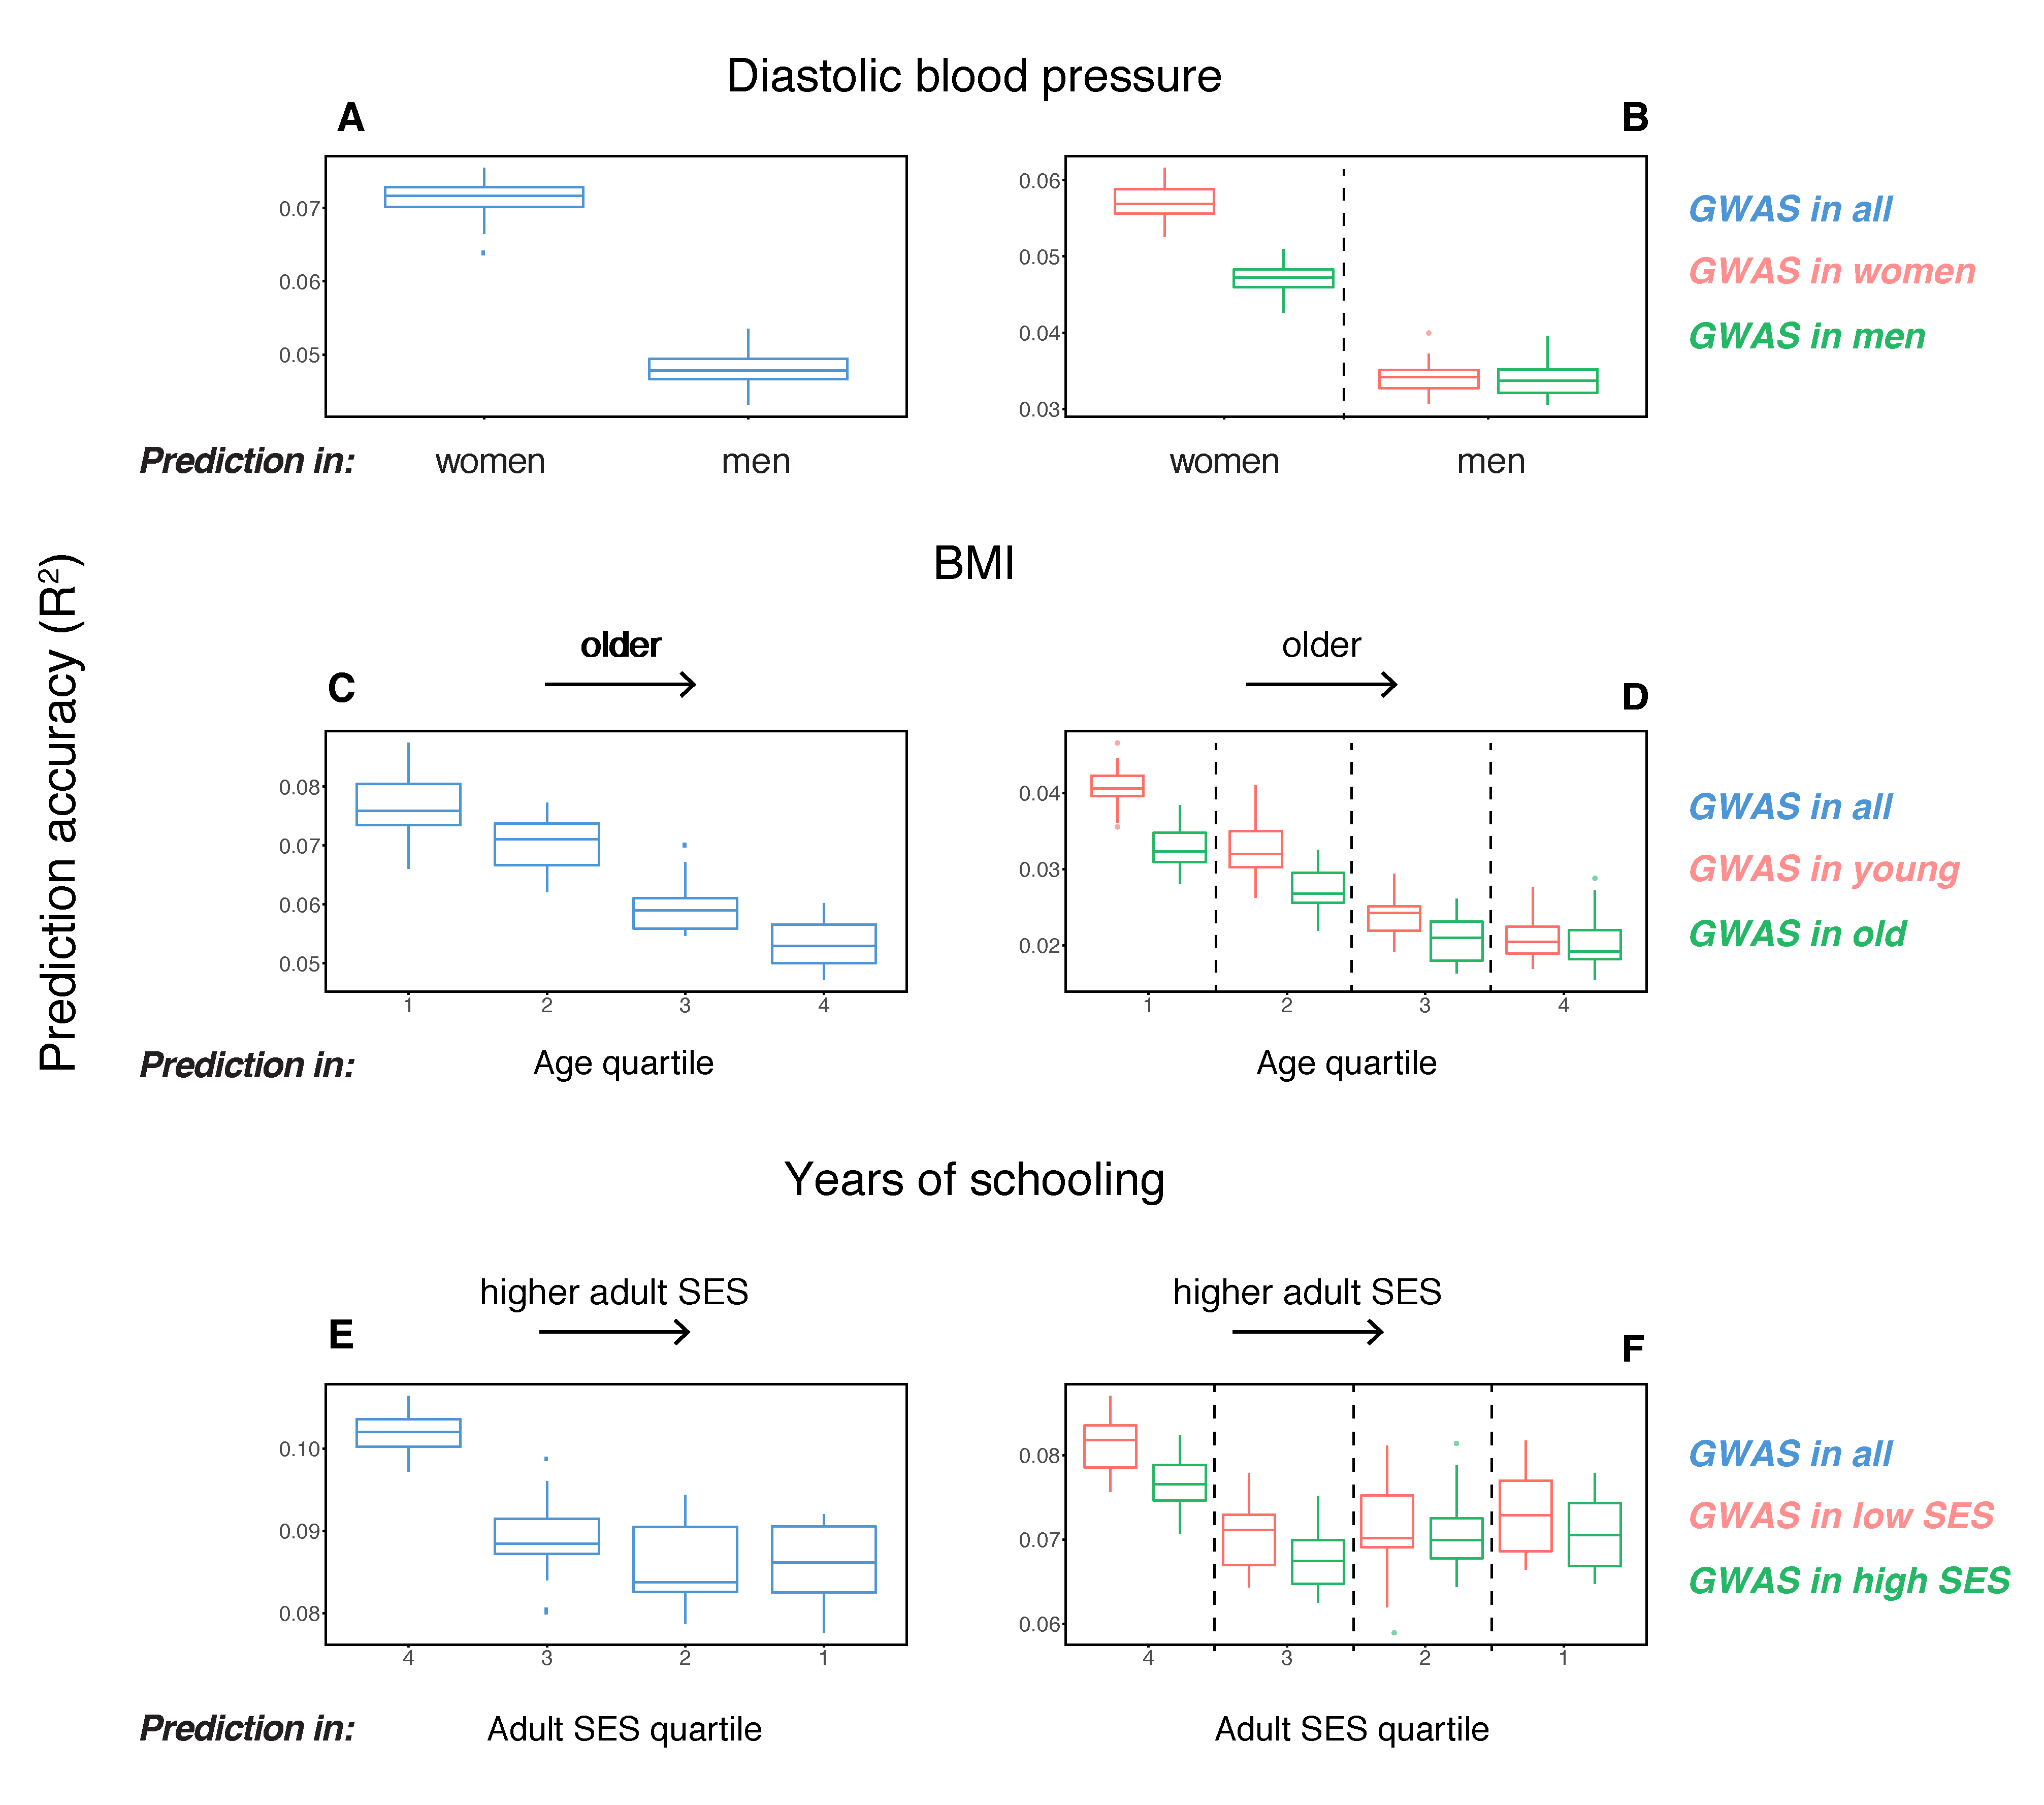
\includegraphics[width=0.7\textwidth]{supp_figures/supp_raw_R2_to_env_boxplot_nice.pdf}
\caption[Variable prediction accuracy (measured as R2) even withn an ancestry group.]{\small Variable prediction accuracy (measured as $R^2$) even withn an ancestry group.  This figure mirrors Fig.~1 of the main text, except for the y-axis showing Shown are $R^2$ values (rather that incremental $R^2$) in different prediction sets. Each box and whiskers plot is computed based on twenty choices of estimation and prediction sets. Thick horizontal lines denote the medians.  {\bf (A,C,E)} The polygenic scores were estimated in large samples of unrelated WB individuals. Phenotypes were then predicted in distinct samples of unrelated WB individuals, stratified by sex (A), age (C) or Townsend deprivation index, a measure of SES (E).  {\bf (B,D,F)} Same as in A,C,E, but here the polygenic scores are based on a GWAS in a sample limited to one sex, age or SES group.  When the GWAS is performed in the group that showed higher prediction accuracy in A,C,E (female, young, low SES), the qualitative trend is the same; but when the GWAS is performed in males, old or high SES, prediction accuracy is diminished and similar across sets.}
\end{figure}


\begin{figure}[!h]
% \label{fig:indirect_simulations}
\centering
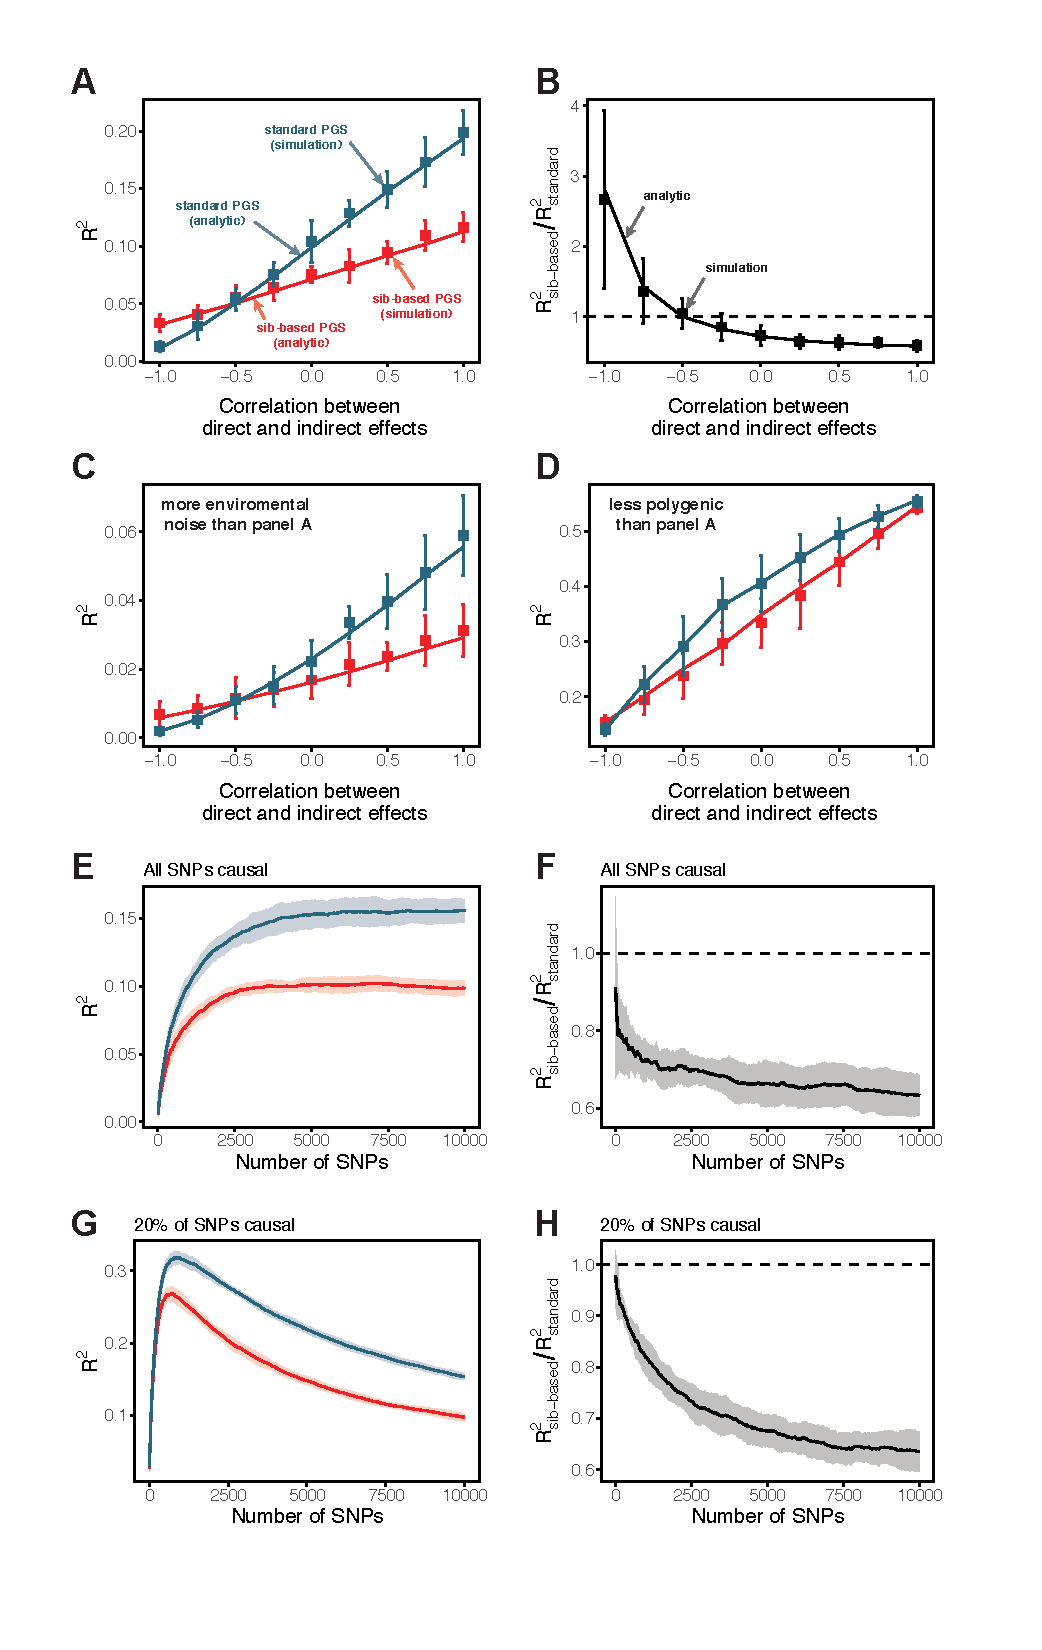
\includegraphics[width=0.7\textwidth]{supp_figures/indirect.pdf}
\caption[Simulation results for standard for sib-based polygenic scores in the presence of indirect effects.]{\small Simulation results for standard for sib-based polygenic scores in the presence of indirect effects.  Simulations were performed with $h_\beta=0.5$ and $h_\eta=0.1$.  The size of the estimation set in the sib GWAS was 15,000, and the size of the estimation set in the standard GWAS was chosen to match estimation noise between the two study designs.  As long as direct and indirect effects are not strongly negatively correlated, out-of-sample prediction accuracy is higher for the standard GWAS-based polygenic scores.}
\label{fig_R_vs_rho_sims}
\end{figure}

\paragraph{Assortative mating.}  We investigate several models of assortative mating by simulation. Standard GWAS-based polygenic scores have greater prediction accuracies than those based on sib regession when parents' phenotypes are positively correlated, and the reverse is true if they are negatively correlated ({\bf Fig.~\ref{fig_assort_mate}A,B}).  Somewhat counter-intuitively, the relative difference in prediction accuracy of the two study designs grows with the inclusion of more SNPs in the polygenic score model ({\bf Fig.~\ref{fig_assort_mate}D,F}).

Throughout, we ignore the ascertainment step where it is decided which SNPs to include in the polygenic score. We assume that SNPs are pre-ascertained and that the set of ascertained SNPs include all causal ones.  We therefore loosely refer to the standard regression on ascertained SNPs (i.e., in a sample of unrelated individuals) and sib regression (regressing difference in phenotypes to difference in sib genotypes) as standard GWAS and sib GWAS, respectively. 
\pagebreak

\begin{figure}[!th]
\centering
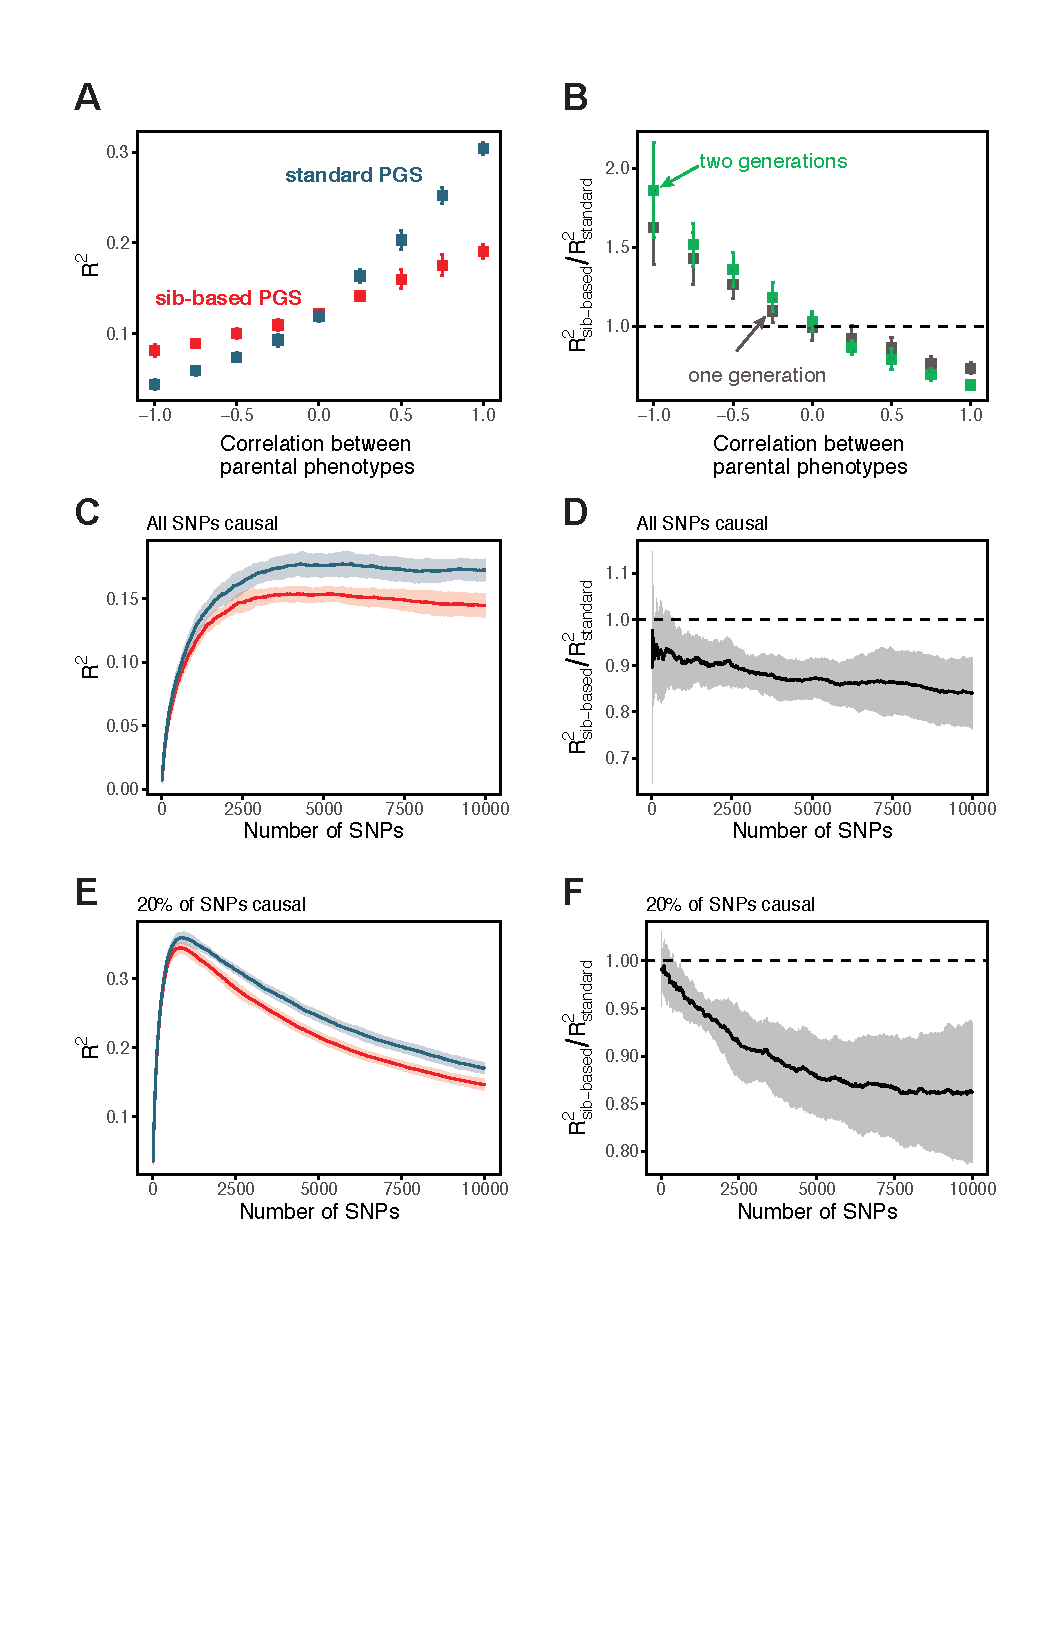
\includegraphics[width=0.7\textwidth]{supp_figures/assort_mate.pdf}
\caption[Prediction accuracy in sib and standard GWAS in the presence of assortative mating.]{\small TBA.}
\label{fig_assort_mate}
\end{figure}

\pagebreak

\subsection{Matching sib-regression and standard GWAS sample sizes}
\label{matching_errors_under_the_null}

We look for the sample size $n^*$ of a standard GWAS performed on sample of unrelated individuals such that, under a simple null model, the resulting polygenic score has the same prediction accuracy out-of-sample as the polygenic score obtained from sib GWAS with sample size $n_{pairs}$.  We begin by assuming that all causal sites $i$ are known and unlinked, and that there is no population stratification or assortative mating.  We  first find the noise associated with estimating the effect size for a single site in each of the two study designs.  We will then examine (and ultimately match) the prediction accuracy of the polygenic scores composed from effect sizes estimated in the estimation sets, $\hat{\beta}_{ur},\hat{\beta}_{sib}$, on a new, independent prediction sample of unrelated individuals $\{(x',y')\}$.

\subsubsection{Error of the estimated effect size at a single site}
Our model for the phenotype value $y$ is
$$y=g+e$$
where $e$ is a Normally distributed environmental effect (including all random noise) and
$$g=\beta^{ur}_0+\sum_{i}\beta_ix_i$$ 
where $x_i \in \{0,1,2\}$ are random genotypes.  The genotype is coded as the effect allele count---the number of alleles with effect $\beta_i$ carried by the individual at site $i$.  We can rewrite our model to focus on the effect size at a single site $i$:
\begin{equation}
\label{ols_model}
y=\beta_0+\beta_ix_i+\epsilon_i,
\end{equation}
where 
$$\epsilon_i=g-\beta_i x_i+e,$$
with variance
$$Var[\epsilon_i]=Var[g-\beta_i x_i]+Var[e] = Var[y]-ֿ\beta_i^2Var[x_i].$$
In OLS regression for the effect of an allele at site $i$, the standard error is
$$Var[\hat{\beta}^{ur}_i]=\frac{Var[\epsilon_i]}{(n-1) Var[x_i^{ur}]} = \frac{Var[y]-ֿ\beta_i^2Var[x_i]}{(n-1)Var[x_i]},$$
where $n$ is the sample size.  In sib GWAS our model for site $i$ is
$$\Delta y=\beta^{s}_0+\beta_i \Delta x_i+\Delta \epsilon_i,$$
with variance
$$Var[\Delta \epsilon_i] = Var[\Delta g-\beta_i \Delta x_i] + Var[\Delta e] =$$
$$Var[\Delta g]+\beta_i^2Var[\Delta x_i]-2\beta_i^2 Var[\Delta x_i]+ Var[\Delta e]$$
Using the $A$ and $B$ subscripts to denote sibs. Recall that for sibs we expect
$$Cov[x_{i,A},x_{i,B}]=\frac{1}{2}Var[x_i],$$
$$Cov[g_A,g_B]=\frac{1}{2}Var[g].$$
Plugging this back in we get
$$Var[\Delta \epsilon_i] = Var[g] - \beta_i^2var[x_i] + 2Var[e](1-\rho_{sibs}) $$
where $\rho_{sibs} = Cor[e_A,e_B]$ is the correlation in environmental effect between sibs. The variance of the estimated effect size in sib GWAS is therefore
$$Var[\hat{\beta}^{s}_i]=\frac{Var[\Delta \epsilon_i]}{(n_{pairs}-1) Var[\Delta x_i]} = \frac{Var[y] - \beta_i^2var[x_i] + Var[e](1-2\rho_{sibs})}{(n_{pairs}-1) Var[x_i]}.$$


\subsubsection{Sample size required for matched prediction accuracy}

We will measure prediction accuracy as the expected correlation between the polygenic score function $\hat{g}$ and the phenotype in an independent prediction set \{(x',y')\},
$$R = \frac{Cov[\hat{g}(x'),y']}{\sqrt{Var[y']Var[\hat{g}(x')}]},$$
by requiring 

\newcommand\reqeq{\mathrel{\stackrel{\makebox[0pt]{\mbox{\normalfont\tiny !}}}{=}}}

$$R(standard~GWAS~with~sample~size~n^*) \reqeq R(sib~regression~with~sample~size~n_{pairs})$$
or equivalently
\begin{equation}
\label{matched_nstar}
\frac{Cov[\hat{g}_{sib}(x'),y']}{\sqrt{Var[\hat{g}_{sib}(x')]}} \reqeq \frac{Cov[\hat{g}_{ur}(x'),y']}{\sqrt{Var[\hat{g}_{ur}(x')]}}.
\end{equation}
We find a sample size $n^*$ to use in the estimator $\hat{g}_{ur}$ that satisfies this condition.  We note that if the vector of estimates $\hat{\beta}$ is given then
$$ Cov[y',\hat{g}(x')|\hat{\beta}]=Cov[g(x'),g(x')]+\sum_i^m{x_i'(\hat{\beta}_i-\beta_i)}|\hat{\beta}] = $$
$$Var[g(x')|\hat{\beta}]+\sum_i^m{Cov[\beta_ix_i',(\hat{\beta}_i-\beta_i)x_i'}|\hat{\beta}]=\sum_i^mVar[x_i']\beta_i\hat{\beta}_i,$$
However, to incorporate the uncertainty both in the estimation set (summarized by the Multivariate Normal distribution of $\hat{\beta}$) and the prediction set (the randomness of $(x',y')$) we will use the law of total covariance,
$$ Cov[y',\hat{g}(x')]=E_{\hat{\beta}}[Cov_{(x',y')}[y',\hat{g}(x')|\{\hat{\beta}\}]]+Cov_{\hat{\beta}}[E_{(x',y')}[Cov[y'|\{\hat{\beta}\}],E_{(x',y')}[\hat{g}(x')|\{\hat{\beta}\}]]=$$
$$E_{\hat{\beta}}\sum_i^mVar[x_i']\beta_i\hat{\beta}_i+Cov_{\hat{\beta}}[\sum_i^mE[x_i']\beta_i,\sum_i^mE[x_i']\hat{\beta}_i]=\sum_i^mVar[x_i]\beta_i^2.$$
Plugging this result back into eq.~\ref{matched_nstar}, we are left with the requirement 
\begin{equation}
\label{matched_nstar_new}
Var[\hat{g}_{sib}(x')] \reqeq Var[\hat{g}_{ur}(x')].
\end{equation}
Applying the law of total variance for each estimated polygenic score $\hat{g}$,
$$Var[\hat{g}_{sib}(x')] =Var_{\hat{\beta}}[E_{x'}[\hat{g}_{sib}(x')|\hat{\beta}]]+E_{\hat{\beta}}[Var_{x'}[\hat{g}_{sib}(x')|\hat{\beta}]] =$$
$$\sum_i^mE[X_i']Var[\hat{\beta}_i]+\sum_i^mVar[X_i']Var[\hat{\beta}_i].$$
Plugging $Var[\hat{g}_{sib}(x')]$ back into \ref{matched_nstar_new} and reordering, 
$$\frac{n^*-1}{n_{sib}-1}=\frac{1}{1+\frac{Var[e](1-2\rho_{sibs})}{Var[y]-\frac{(\sum_i^mE[x_i^2]\beta_i^2)}{(\sum_i^m\frac{E[x_i^2]}{Var[x_i]})}}},$$
or, assuming 
$$\frac{(\sum_i^mE[x_i^2]\beta_i^2)}{(\sum_i^m\frac{E[x_i^2]}{Var[x_i]})} << Var[y],$$ 
%\hl{there's probably a nicer way to present this assumption. but should be a valid assumption}
we find
\begin{equation}
\label{final_nstar_just_direct}
\frac{n^*}{n^{pairs}} \approx \frac{1}{1+(1-h_{\beta}^2)(1-2\rho_{sibs})}.
\end{equation}

eq.~\ref{final_nstar_just_direct} can be adopted, in principle, for the estimation of $\rho_{sibs}$ for different traits---under our model assumptions, and given an independent estimate of $h_{\beta}^2.$

\subsubsection{Empirical matching of standard errors}
\label{Empiricalmatchingofstandarderrors}
The result of eq.~\ref{final_nstar_just_direct} is the same as we would obtain if we required 
\begin{equation}
\label{requirement_just_estimation_set}
\forall i~Var[\hat{\beta}_i^{sib}(x_i)] \reqeq Var[\hat{\beta}_i^{ur}(x_i^{sib})]
\end{equation}
without taking  into account randomness in the prediction set.  In practice (and in the results shown in the main text), we have no prior knowledge on $\rho_{sibs}$ and instead we find a sample size $n^*$ for the standard GWAS such that
\begin{equation}
\label{requirement_median}
median_i(Var[\hat{\beta}_i^{sib}(x)]) \reqeq median_i(Var[\hat{\beta}_i^{ur}(x)])
\end{equation}
We note that the condition in eq.~\ref{requirement_just_estimation_set} is approximately met because, if we assume that $y$ is a highly polygenic trait where
$$ \forall i~\beta_i^2Var[xi] << Var[y],$$
then 
$$\forall i~Var[\hat{\beta}_i^{sib}(x)]=Var[\hat{\beta}_i^{ur}(x)]=\frac{D}{Var[x_i]}$$
where D is the same for sib- and standard GWAS estimates (given that a sample of $n^*$ is used), and approximately independent of $\beta_i$.  eq.~\ref{requirement_median} can be thought of as a weighted-median of D. In conclusion, the requirement of eq.~\ref{requirement_median} leads to equal prediction accuracy under the null model assumptions.

\pagebreak

\subsection{Indirect parental effects}
\subsubsection{Distribution of effect estimate at a single site}
We consider a model with direct effects, as well as indirect parental effects, assuming no interaction between parents and the polygenic score of the children and ignoring possible indirect effects of sibs on each other.
We start by considering the model
$$y=\beta_0+g+n+e$$
where g is the sum of direct effects in an individual with genotypes (effect-allele count) $x_i$ at each site $i$,
$$g=\sum_i^m\beta_ix_i,$$ 
and 
$$n=\sum_i^m\eta_i(x_i+\tilde{x}_i^m+\tilde{x}_i^p)$$ 
is the sum of parental indirect effects to the phenotype, with parental allele counts $x_i+\tilde{x}_i^p+\tilde{x}_i^m$ at each site where $\tilde{x}_i^m$ is the untransmitted maternal effect allele count, and $\tilde{x}_i^p$ is the untransmitted paternal effect allele count, with $\tilde{x}_i^m,\tilde{x}_i^p \in \{0,1\}$.  As we show, when we match the errors of the estimated effect sizes of a standard GWAS then the prediction accuracy of the two polygenic scores differ in an independent sample: unless there is a large negative correlation between indirect and direct effects, the polygenic score from standard GWAS is expected to outperform the one based on sibs.

We first examine the distribution of an estimated effect size of $x_i$ on the phenotype.  The OLS regression for a single site in a standard GWAS follows eq.~\ref{ols_model} and can be rewritten as
\begin{equation}
\label{OLS_indirect}
y=\beta_0+(\beta_i+\eta_i)x_i+\eta_i(\tilde{x}_i^p+\tilde{x}_i^m)+\epsilon_i
\end{equation}
with
$$\epsilon_i=g+n+e-(\beta_i+\eta_i)x_i-\eta_i(\tilde{x}_i^p+\tilde{x}_i^m).$$
By the assumption of no assortative mating or other population structure,
\begin{equation}
\label{no_assort_or_structure}
Cov[\tilde{x}_i^p,\tilde{x}_i^m]=Cov[x_i,\tilde{x}_i^m]=Cov[x_i,\tilde{x}_i^p]=0.
\end{equation}
It directly follows that in eq.~\ref{OLS_indirect} we have two terms involve independent variables.  Therefore,  $\hat{\beta^{ur}}_i$ is Normally distributed and unbiased, with expectation 
$$E[\hat{\beta}_i]=\beta_i+\eta_i.$$
We next calculate $\hat{\beta}_i^{ur}$'s variance. From assumption \ref{no_assort_or_structure} and 
$$Var[\tilde{x}_i^m+\tilde{x}_i^p]=Var[x_i],$$
we obtain
$$Var[\epsilon_i]=Var[y]+(\beta_i+\eta_i)^2Var[x_i]+\eta_i^2Var[x_i]-2Cov[g+n,(\beta_i+\eta_i)x_i]-2Cov[n,\eta_i(\tilde{x}_i^m+\tilde{x}_i^p)]=$$
$$=Var[y]-Var[x_i] (\beta_i^2+2\beta_i \eta_i + 2 \eta_i^2).$$
Finally,
$$Var[\hat{\beta}_i^{ur}]=\frac{Var[\epsilon_i]}{(n-1)Var[x_i]}=\frac{Var[y]-Var[x_i] (\beta_i^2+2\beta_i \eta_i + 2 \eta_i^2)}{(n-1)Var[x_i]}.$$
In sib regression, we have
$$\Delta y=\Delta g+\Delta e$$
as indirect parental effects cancel out when taking the difference between sibs, because the sibs have an equal parental effect allele count. Thus, the expected estimate is the same it was in the absence of direct effects;  Using the same considerations for the variance of sib differences as in {\bf Section \ref{matching_errors_under_the_null}}, we obtain    
$$\hat{\beta}_i^{sib} \sim N(\beta_i,\frac{Var[g] - \beta_i^2var[x_i] + Var[e](1-2\rho_{sibs})}{(n_{pairs}-1) Var[x_i]}),$$
where $\rho_{sibs}$ is again the correlation in environmental effect between sibs.

\subsubsection{Polygenic score prediction accuracy}
We now examine the difference in prediction accuracy of $\hat{g}^{ur}$ and $\hat{g}^{sib}$ after matching 
\begin{equation}
\label{matching_errors_indirect}
Var[\hat{\beta}_i^{ur}] \reqeq Var[\hat{\beta}_i^{sib}]
\end{equation}
by choosing a standard GWAS sample size $n^*$ that empirically satisfies the condition, as we do in the main text (see also section \ref{Empiricalmatchingofstandarderrors}).  
% By this approach, we obtain
% $$ Cov[y',\hat{g}(x')]=\sum_i^m(\beta_i+\eta_i)Cov[\hat{\beta}_ix_i',x_i']+\eta_iCov[\hat{\beta}_ix_i',(\tilde{x}_i'^m+\tilde{x}_i'^p)].$$
% Taking eq.~\ref{no_assort_or_structure} into account, the second term is zero.  By the law of total covariance,
% $$ Cov[y',\hat{g}(x')]=\sum_i^m(\beta_i+\eta_i)E_{\hat{\beta}}[Cov_{x'}[\hat{\beta}_ix_i',x_i']|\hat{\beta}]+\sum_i^m(\beta_i+\eta_i)Cov_{\hat{\beta}}[E_{x'}[\hat{\beta}_ix_i'|\hat{\beta}],E_{x'}[x_i']|\hat{\beta}]]=$$
% $$=\sum_i^m(\beta_i+\eta_i)E_{\hat{\beta}}[Var[x_i]\hat{\beta}_i]+\sum_i^m(\beta_i+\eta_i)Cov_{\hat{\beta}}[\hat{\beta}_iE[x_i'],E[x_i']],$$
% \begin{equation}
% \label{covariance_prediction}
% =\sum_i^mVar[x_i](\beta_i+\eta_i)E[\hat{\beta}_i].
% \end{equation}
% Similarly, by the law of total variance,
% $$Var[\hat{g}(x')] =Var_{\hat{\beta}}[E_{x'}[\hat{g}(x')|\hat{\beta}]]+E_{\hat{\beta}}[Var_{x'}[\hat{g}(x')|\hat{\beta}]] = Var_{\hat{\beta}}[\sum_i^m\hat{\beta}_iE[x_i]]+E_{\hat{\beta}}[\sum_i^mVar[x_i]\hat{\beta}_i^2]=$$
% \begin{equation}
% \label{variance_ps_prediction}
% \sum_i^mE[x_i]^2Var[\hat{\beta}_i]+\sum_i^mVar[x_i]E[\hat{\beta}_i^2].
% \end{equation}
% Taken together, eq.~\ref{covariance_prediction} and eq.~\ref{variance_ps_prediction} give
We can derive the expected prediction accuracy by averaging over both the estimation set (which we again shorthand as the distribution of $\hat{\beta}$) and the prediction set ${x',y'}$.  By the law of total expectation,
\begin{equation}
\label{total_expectation_for_R2}
E[R^2] = E_{\hat{\beta}}[E_{x'}[R^2]] \approx 
\frac{E_{\hat{\beta}}[Cov_{x'}[\hat{g}(x'),y'|\hat{\beta}]]}{E_{\hat{\beta}}[Var_{x'}[y']E_{\hat{\beta}}[Var_{x'}[\hat{g}(x')|\hat{\beta}]},
\end{equation}
where we approximate the expected prediction accuracy by its first-order Taylor expansion.  The numerator  of eq.~\ref{total_expectation_for_R2} is 
\begin{equation}
\label{E_cov_y'_g_hat}
E_{\hat{\beta}}[Cov_{x'}[\hat{g}(x'),y'|\hat{\beta}]]=\sum_i^m(\beta_i+\eta_i)E_{\hat{\beta}}[Cov_{x'}[\hat{\beta}_ix_i',x_i']|\hat{\beta}] = \sum_i^m Var[x_i](\beta_i+\eta_i)E[\hat{\beta}_i],
\end{equation}
and the denominator terms are 
\begin{equation}
\label{E_Var_y'}
E_{\hat{\beta}}[Var_{x'}[y'|\hat{\beta}]] = Var[y]
\end{equation}
and
\begin{equation}
\label{E_var_g_hat}
E_{\hat{\beta}}[Var_{x'}[\hat{g}(x')|\hat{\beta}] = E_{\hat{\beta}}[\sum_i^mVar[x_i]\hat{\beta}_i^2] =
\sum_i^mVar[x_i](E[\hat{\beta}_i]^2+Var[\hat{\beta}_i]).
\end{equation}

Plugging eq.~\ref{E_cov_y'_g_hat},\ref{E_Var_y'},\ref{E_var_g_hat} back into eq.~\ref{total_expectation_for_R2} we obtain

% $$\frac{\sum_i^mVar[x_i](\beta_i+\eta_i)E[\hat{\beta}_i]}{\sqrt{Var[y]}\sqrt{\sum_i^mE[x_i]^2Var[\hat{\beta}_i]+\sum_i^mVar[x_i]E[\hat{\beta}_i^2]}} =$$
\begin{equation}
\label{R_indirect_general_form}
E[R^2] \approx \frac{(\sum_i^mVar[x_i](\beta_i+\eta_i)E[\hat{\beta}_i])^2}{Var[y](\sum_i^mVar[x_i]Var[\hat{\beta}_i]+\sum_i^mVar[x_i]E[\hat{\beta}_i]^2)}
\end{equation}
We next note that 
$$\tilde{C}:=Var[y]\sum_i^m Var[x_i] Var[\hat{\beta}_i]$$
is the same for sib regression and standard GWAS under the requirement of eq.~\ref{matching_errors_indirect}.  We therefore have 
\begin{equation}
\label{R_indirect_unrelated_longform}
E[R_{ur}^2] \approx \frac{(\sum_i^mVar[x_i](\beta_i+\eta_i)^2)^2}{\tilde{C}+ Var[y]\sum_i^mVar[x_i](\beta_i+\eta_i)^2},
\end{equation}
and
\begin{equation}
\label{R_indirect_sibs_longform}
E[R_{sib}^2] \approx \frac{(\sum_i^mVar[x_i](\beta_i+\eta_i)\beta_i)^2}{\tilde{C}+ Var[y]\sum_i^mVar[x_i]\beta_i^2}.
\end{equation}

If we denote the heritability explained by direct effects by
$$h_{\eta}^2:=\frac{\sum_i^mVar[x_i]\beta_i^2}{Var[y]},$$
the heritability explained by indirect effects by
$$h_{\beta}^2:=\frac{\sum_i^mVar[x_i]\eta_i^2}{Var[y]},$$
and the heritability explained by both direct and indirect effects by
$$h^2:=\frac{\sum_i^mVar[x_i](\beta_i+\eta_i)^2}{Var[y]}$$
then the square of eq.~\ref{R_indirect_unrelated_longform} can be written as
\begin{equation}
\label{R_indirect_unrelated_shortform}
E[R_{ur}^2] \approx h^2\frac{1}{1+c},
\end{equation}
where we defined
$$c:=\frac{\sum_i^mVar[x_i]Var[\hat{\beta}_i]}{\sum_i^mVar[x_i](\beta_i+\eta_i)^2}.$$
Here, $c$ can be thought of as a summary of estimation noise, i.e., a weighted average of the coefficients of variation of effect size estimators.
If we further assume that effects are randomly distributed across sites and are iid  (implying, in particular, that effect sizes and allele frequencies are independent),
\[ 
\left (
  \begin{tabular}{c}
  \beta_i \\
  \eta_i
  \end{tabular}
\right ) \sim
\left ( \left (
  \begin{tabular}{c}
  0 \\
  0
  \end{tabular}
\right ),
\left (
  \begin{tabular}{cc}
  \sigma_\beta^2 & \rho \sigma_\beta \sigma_\eta  \\
  \rho \sigma_\beta \sigma_\eta & \sigma_\eta^2 
  \end{tabular}
\right )\right ), 
\] then the expectation of the numerator of eq.~\ref{R_indirect_sibs_longform} is
$$E_{\beta,\eta}[\sum_i^mVar[x_i]\beta_i(\beta_i+\eta_i)]=\sum_i^mVar[x_i]E_{\beta_i,\eta_i}[\beta_i^2+\beta_i \eta_i]=\sum_i^mVar[x_i](\sigma_{\beta}^2+\rho \sigma_{\beta} \sigma_{\eta})$$
thus eq.~\ref{R_indirect_sibs_longform}, in expectation, is:

\begin{equation}
\label{R_indirect_sibs_shortform}
E[R_{sib}^2] \approx (1+\rho \frac{\sigma_\eta}{\sigma_\beta})^2 h_\beta^2 \frac{1}{1 + c/\alpha}.
\end{equation} where
$$\alpha := h_\beta^2 / h^2=  \frac{\sum_i^mVar[x_i]\beta_i^2}{\sum_i^mVar[x_i](\beta_i+\eta_i)^2}.$$

We examined the fit of this prediction to simulated data.  Specifically, we ran simulations to estimate effect sizes in a sib-GWAS and in a standard GWAS, after choosing $n^*$ to match their variances.  Finally, we predicted phenotypes in a sample of unrelated individuals (see {\bf Section \ref{indirect_sim_details}} for further detail).

{\bf Fig.~\ref{fig_R_vs_rho_sims}} shows the the analytic result alongside simulation results for different correlation coefficients between indirect and direct effect sizes.  Even in the absence of correlation between indirect and direct effect sizes, the polygenic score based on standard GWAS outperforms the sib-based polygenic score.  

To understand this behavior and dependency of the $\frac{R_{sib}^2}{R_{ur}^2}$ ratio on other parameters, we divide eq.~\ref{R_indirect_sibs_shortform} by eq.~\ref{R_indirect_unrelated_shortform} and obtain
$$E[\frac{R_{sib}^2}{R_{ur}^2}] \approx \left(1+\rho \frac{\sigma_{\eta}}{\sigma_{\beta}}\right)^{2}\alpha \frac{1+c}{1+c/\alpha}.$$
Noting further that
$$\left(1+\rho \frac{\sigma_{\eta}}{\sigma_{\beta}}\right)^{2} \alpha=\left(\frac{\sigma_\beta+\rho \sigma_\eta}{\sigma_\beta}\right)^{2} \frac{\sigma_\beta^{2}}{\sigma_\beta^{2}+2 \rho \sigma_{\beta} \sigma_{\eta}+\sigma_{\eta}^{2}}=1-(1-\rho^2)\frac{h_\eta^2}{h^2},$$
we get
\begin{equation}
\label{R2_ratio}
E[\frac{R_{sib}^2}{R_{ur}^2}] \approx [ 1-(1-\rho^2) \frac{h_\eta^2}{h^2}]\frac{1+c}{1+c\frac{h^2}{h_\beta^2}}.
\end{equation}

A few conclusions emerge from eq.~\ref{R2_ratio}.  First, the sib-based polygenic score will outperform the standard polygenic score only if direct and indirect effects are strongly negatively correlated.   Second, the term
$$\frac{1+c}{1+c\frac{h^2}{h_\beta^2}}=\frac{1+\frac{\sum_i^mVar[\hat{\beta}_i]Var[x_i]}{h^2}}{1+\frac{\sum_i^mVar[\hat{\beta}_i]Var[x_i]}{h_{\beta}^2}}$$
can be though of the dependence on the noise-to-signal ratio (the signal being the total heritability and the direct-effect heritability); for a given estimation noise (matched across the two study designs), we get a different amount of signal from standard and sib-GWAS.  Importantly, we note that random estimation noise factors into the expected prediction accuracies ratio.  If indirect nurture does not exist, or has negligible effects on the trait in question, the prediction accuracies ratio is expected to be one.  However, in the presence of indirect effects, the magnitude of the deviation from 1 depends on the relationship between heritability components (direct, indirect and their covariance) as well as on the (matched) estimation noise.

%\hl{discussion behavior, limit behavior and figure illustrating behavior}

%\hl{discussion of effect of p-value threshold, alongside simulations that include the ascertainment of SNPs}

\vspace{0.5cm}

%This is because in this case $\alpha < 1$.  This is true as long as $c$ is nonzero (it approaches zero for very large estimation sample sizes). For realistic sample sizes, however, $c$ is nonzero.  As Fig.~\ref{fig_R_vs_rho_sims} demonstrates, unless the indirect and direct effects are strongly negatively correlated ($<0.5$), prediction accuracy will be higher using the standard GWAS with unrelated individuals.\\

\subsubsection{Indirect effects simulation details}
\label{indirect_sim_details}
For each set of individuals used for estimation or prediction, we first simulated mother-father pairs, assigning parental alleles as $Bernoulli(p_i)$, where $p_i$ denotes the effect allele frequency at site $i$.  We then sampled the parental alleles to generate offspring (one offspring per each mother-father pair to simulate a sample of unrelated individuals, and two offspring to generate sibling pairs). Phenotypes of the offspring were sampled from a Normal distribution with mean
$$\sum_i^m\beta_ix_i+\eta_i({x}_i^p+{x}_i^m)$$ (where ${x}_i^m$ and ${x}_i^p$ are the maternal and paternal effect allele counts, respectively) and variance 
$$1-h^2.$$
Using this approach, we generated a set a of sibling pairs and estimated SNP effect sizes using a sibling regression. We then calculated $n^*$ as follows: we simulated sets of unrelated individuals with a range of sample sizes. In each set, we performed simple linear regression of phenotype to genotype.  We then estimated a linear relationship between the inverse of the median standard error of effect size estimates (as a dependent variable) and the square root of the sample size.  Using this linear relationship, we then predicted the sample size for the unrelated set that gives a median standard error equal to the median standard error of sib-regression effect size estimates ($n^*$).  Finally, we simulated a set of unrelated individuals with sample size $n^*$ and compared the prediction accuracy ($R^2$) of the polygenic score based on this sample and the sib-based polygenic score. 

In these simulations, we used the following parameter values:

- ratio of the heritability accounted for by direct effects versus indirect effects: 5

- heritability from direct effects: 0.5

- allele frequencies are drawn from a truncated exponential distribution, truncated on the left such that the minimum allele frequency is 1\%.

- number of loci: 1000.

- Variance of direct effect size: 1.

- Variance of indirect effect size: 0.25.

- number of sibling pairs for sib GWAS: 13,000

- number of unrelated individuals for prediction: 20,000

- one iteration was used to estimate $n^*$ and $R$ for a given $\rho$ (i.e., correlation between direct and indirect effect sizes) and heritability ratio.


\pagebreak

\subsection{Assortative mating}
We considered assortative mating with regard to a phenotype, whereby the mating of individuals in the population is dependent on the degree of their similarity with respect to that phenotype.  This process generates a correlation (linkage disequilibrium) between genetic variants that contribute to the phenotype.  Consequently, in a standard GWAS, the marginal effect sizes of causal SNPs will partially capture the effect size of other causal SNPs as well. Thus, estimated effect sizes are expected to be inflated under positive assortative mating (mating of similar individuals) and deflated under negative assortative mating (mating of dissimilar individuals). In turn, in a sibling-based GWAS, the estimates are in expectation unaffected by assortative mating, because genetic differences between siblings arise from random Mendelian segregation in the parents. 

\subsubsection{Assortative mating simulations}
We used simulations to examine the phenotypic prediction accuracies of sibling-based and standard polygenic scores in a sample of unrelated individuals under a model with assortative mating, varying the correlation between parental phenotypes $\rho_a$. Similar to our simulations for indirect effects ({\bf Section~\ref{indirect_sim_details}}), we first simulated the estimation procedure in a sibling-based and in a standard GWAS (with sample size $n^*$). We then computed the prediction accuracy $R^2$ in an independent sample of unrelated individuals (see {\bf Further simulation details} below).\\

We first considered the simple case of a single generation of assortative mating. In the presence of positive assortative mating ($\rho_a>0$) standard polygenic scores based on unrelated samples outperform sib-based polygenic scores, whereas the opposite is true in the case of negative assortative mating ($\rho_a<0$) ({\bf Fig.~\ref{fig_assort_mate}A}). In simulations of two generations of assortative mating, the gap between prediction accuracies of standard and sib-based predictions ({\bf Fig.~\ref{fig_assort_mate}B}) is amplified, suggesting that our qualitative findings apply to scenarios of sustained assortative mating as well. We further investigated prediction accuracy as a function of the number of SNPs included in the polygenic scores, progressively adding SNPs, with p-values obtained from an independent GWAS in unrelated samples (similar to our analysis in {\bf Fig. 3}). We considered two genetic architectures scenarios, (i) in which all SNPs are causal and (ii) the case in which 20\% of of SNPs are causal (leading polygenic scores to include non-causal SNPs due to estimation noise). Under both scenarios, the gap in prediction accuracies between standard and sib-based grows with the number SNPs ({\bf Fig.~\ref{fig_assort_mate}C-F}).\\

\paragraph{Further simulation details.}
\label{assortative_sim_details} 
We simulated parental and offspring alleles as described for indirect effects in {\bf Section \ref{indirect_sim_details}}. To simulate assortative mating between parents, we first simulated iid genotypes (effect allele counts $x_i$ at each SNP $i$) and randomly assigned "mother" and "father" labels to each individual. We then generated corresponding parental phenotypes as
$$N(\sum_i^m\beta_ix_i,\sqrt{1-h^2})$$ where  $\beta_i$ is the effect size of SNP $i$, and $h^2$ is the heritability.  The same model was used later to generate offspring phenotypes.

We paired mothers and fathers as follows: we generated a random matrix  
\[ 
\left (
  \begin{tabular}{c}
  $u_{m,i}$ \\
  $u_{p,i}$
  \end{tabular}
\right ) \sim N
\left ( \left (
  \begin{tabular}{c}
  $\overline{y}_m$ \\
  $\overline{y}_p$
  \end{tabular}
\right ),
\left (
  \begin{tabular}{cc}
  $\sigma_{y_m}^2$ & $\rho_a \sigma_{y_m} \sigma_{y_p}$  \\
  $\rho_a \sigma_{y_m} \sigma_{y_p}$ & $\sigma_{y_p}^2$ 
  \end{tabular}
\right )\right ), 
\] where $\overline{y}_m$ and $\overline{y}_p$ are the average phenotypes of mothers and fathers, respectively, $\sigma_{y_m}$ and $\sigma_{y_p}$ are the sample standard errors of the phenotypes of mothers and fathers, respectively, and $\rho_a$ is the desired correlation between parental phenotypes.  We then reordered mothers and fathers sets to match the order of $u_m$ and $u_p$, respectively. In the case of two generations of assortative mating, we similarly simulated the generation of the grandparents.\\

[repeats a lot of the above no?] We compared the performance of standard and sibling-based polygenic scores using the same procedure as described in {\bf Section \ref{indirect_sim_details}}. We additionally investigated the effect of the number of SNPs included in the polygenic scores. For this analysis, we sorted the SNPs based on the association p-value obtained in an independent simulated set of unrelated individuals.\\ 

In the simulations, we used the following parameter values:

- heritability under random mating: 0.5

- number of loci, assumed independent (i.e., in linkage equilibrium) under random mating: 10,000

- number of causal loci: 2,000 or 10,000

- allele frequencies, $p$, drawn from a truncated exponential distribution, truncated on the left such that the minimum allele frequency is 1\%.

- SNP effect sizes set to 0 for non-causal loci and drawn as $\beta_i\sim N(0,\sigma^2)$, choosing $\sigma^2$ to satisfy $\sum_i^m2\beta_i^2p_i(1-p_i)=h^2$ for causal loci. 

- number of sibling pairs for sib GWAS: 10,000

- number of unrelated individuals for prediction: 10,000

- number of unrelated individuals for discovery GWAS (i.e. SNP prioritization): 20,000

- 10 iterations were used to estimate $n^*$ and $R$ for a given $\rho_a=$ (i.e., correlation between parental phenotypes).

\pagebreak

\begin{figure}[h!]
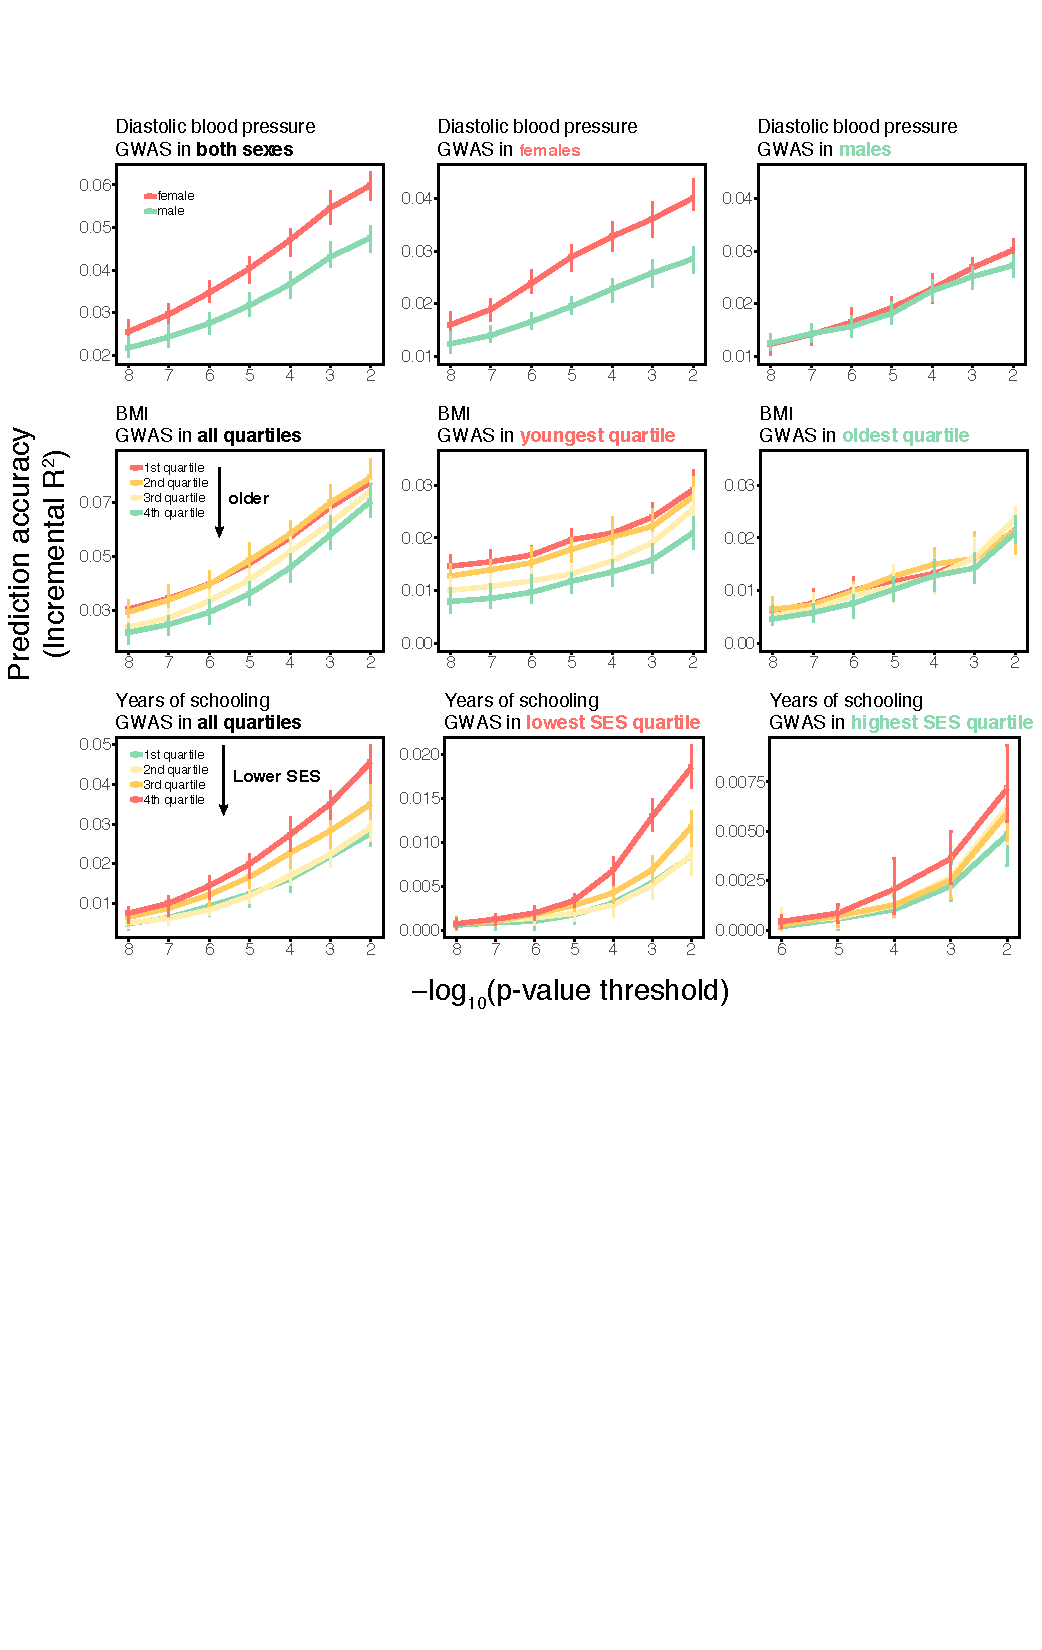
\includegraphics[width=\textwidth]{./supp_figures/fig1_Rsweep.pdf}
\caption{p-value threshold dependence of trends in Fig. 1}
\centering
\end{figure}

\begin{figure}[h!]
\centering
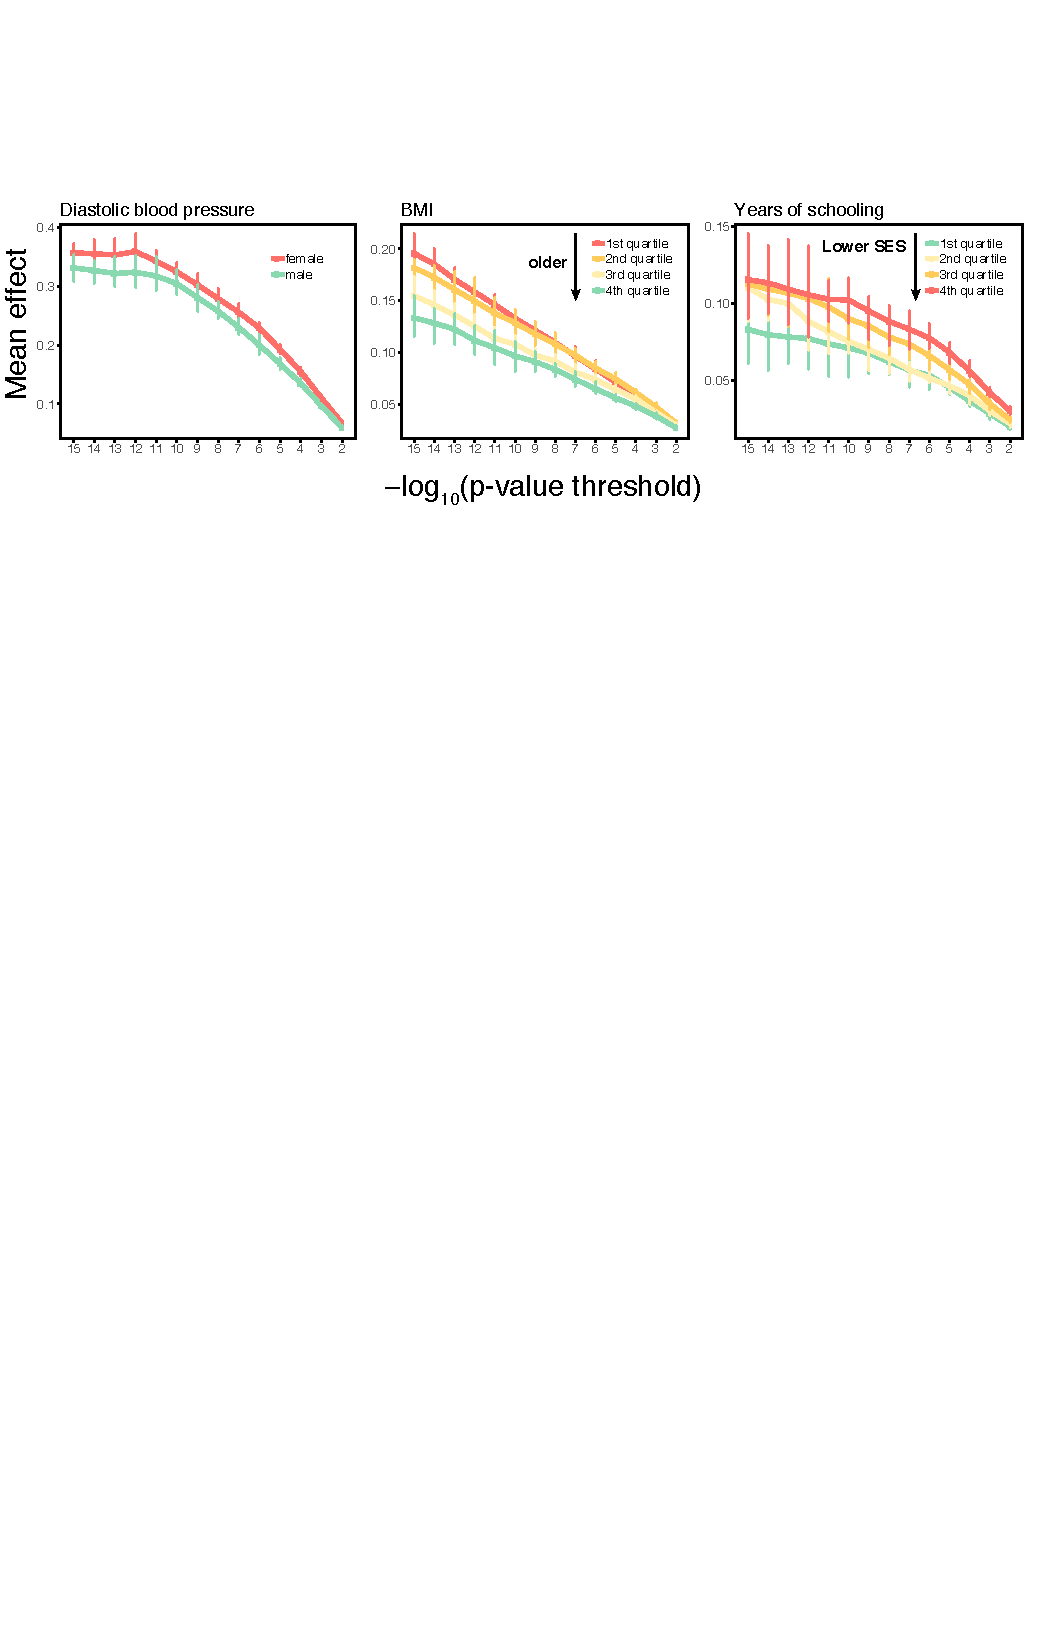
\includegraphics[width=\textwidth]{./supp_figures/beta_sweep.pdf}
\caption{Effects across strata}
\end{figure}


\begin{figure}[h!]
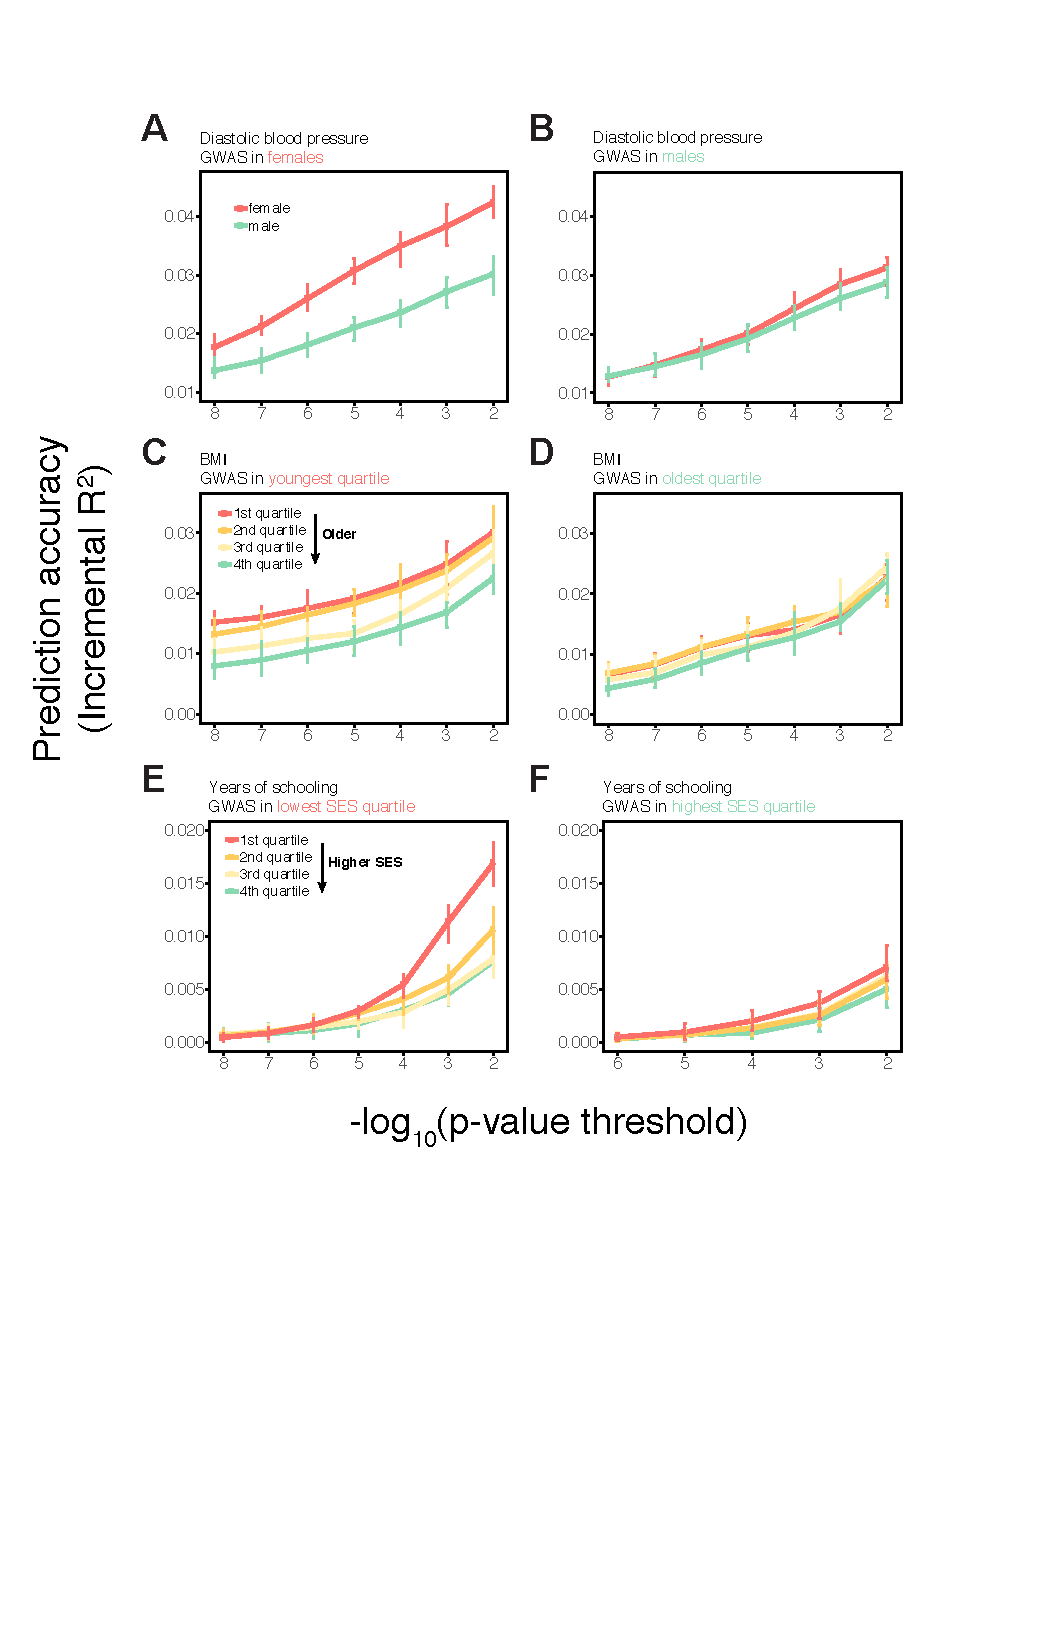
\includegraphics[width=0.9\textwidth]{./supp_figures/bolt.pdf}
\caption{LMM}
\centering
\end{figure}


\begin{figure}[h!]
\centering
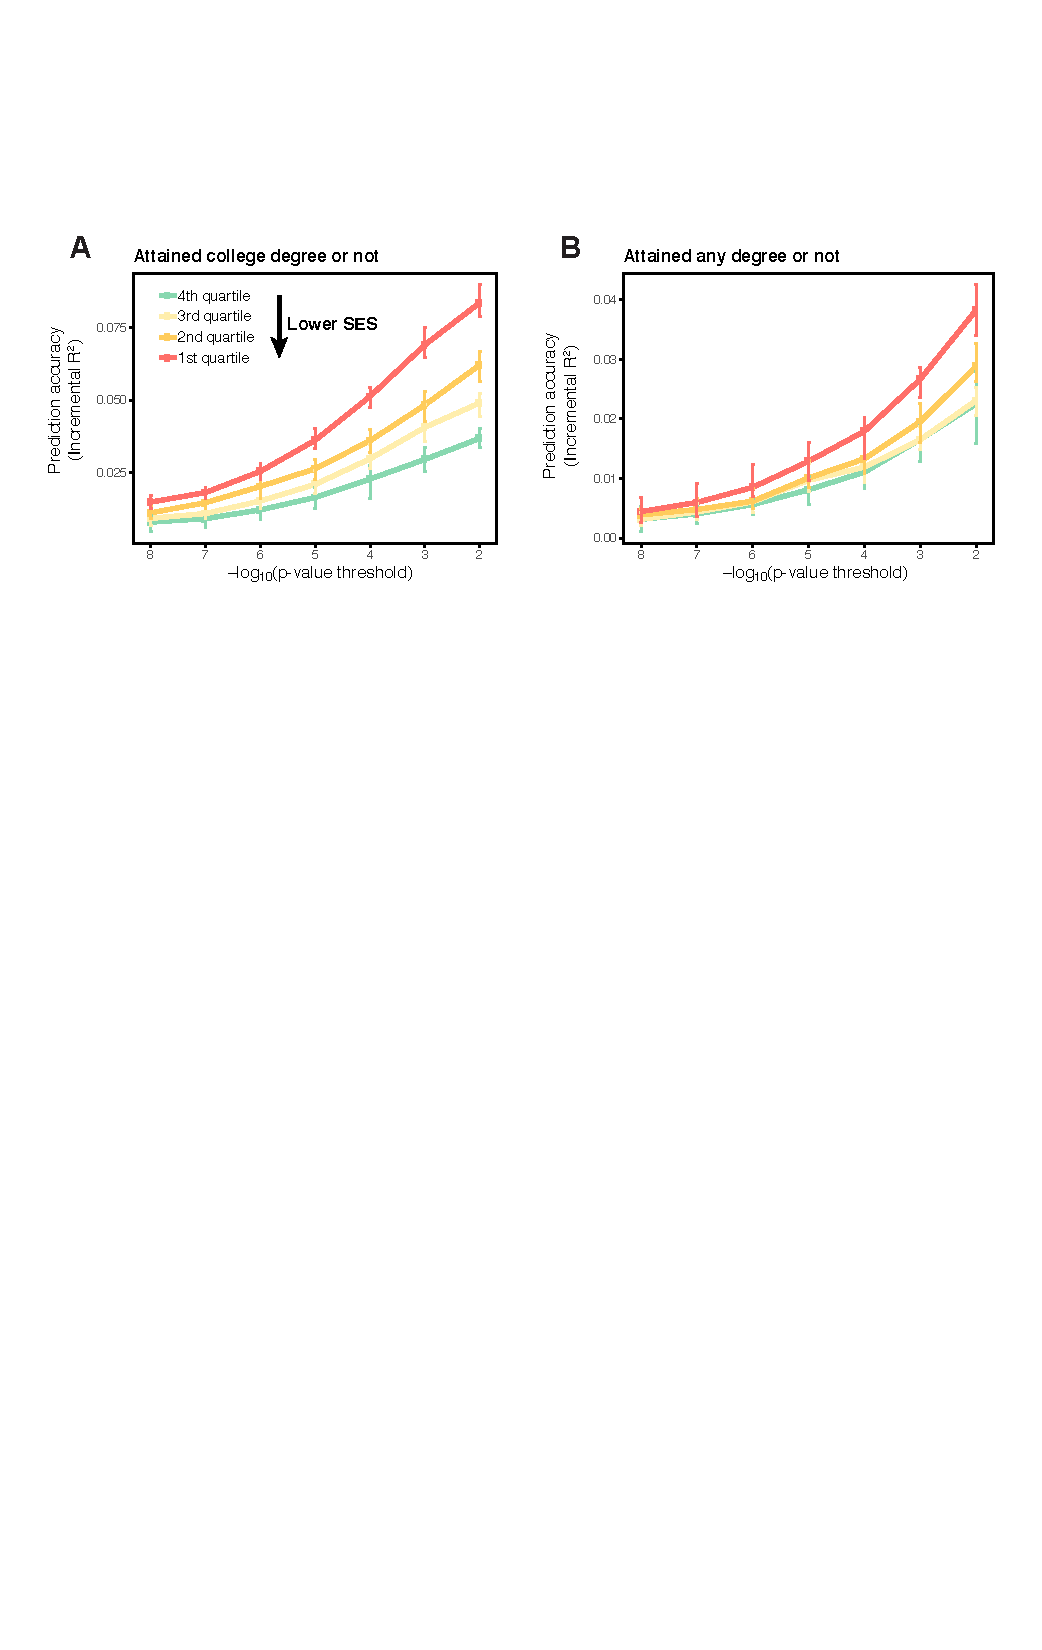
\includegraphics[width=\textwidth]{./supp_figures/binary_edu_traits.pdf}
\caption{Binary education traits}
\end{figure}


\begin{figure}[h!]
\centering
\includegraphics[width=\textwidth]{./supp_figures/Fig3_si_v2.pdf}
\caption{p-value dependence of sib vs standard PS prediction accuracy}
\end{figure}

\begin{figure}[h!]
\centering
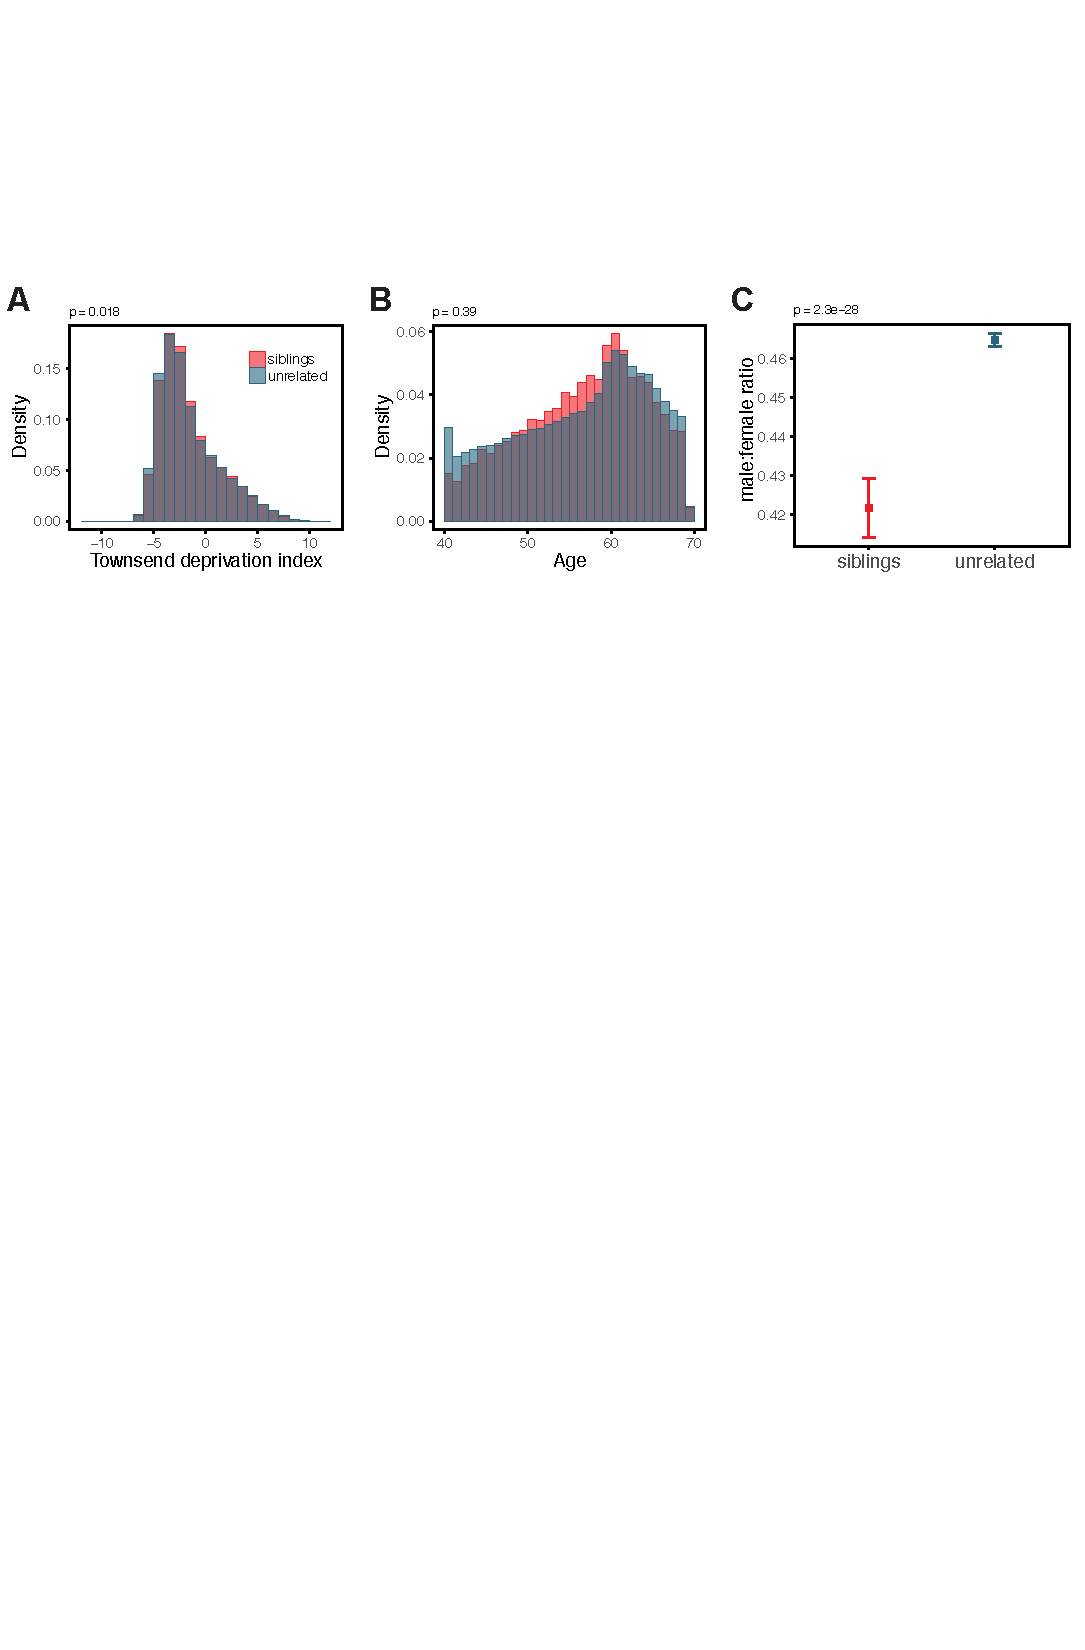
\includegraphics[width=\textwidth]{./supp_figures/sibs_unrel_compare1.pdf}
\caption{sibs vs unrel: age, ses, sex ratio}
\end{figure}

\begin{figure}[h!]
\centering
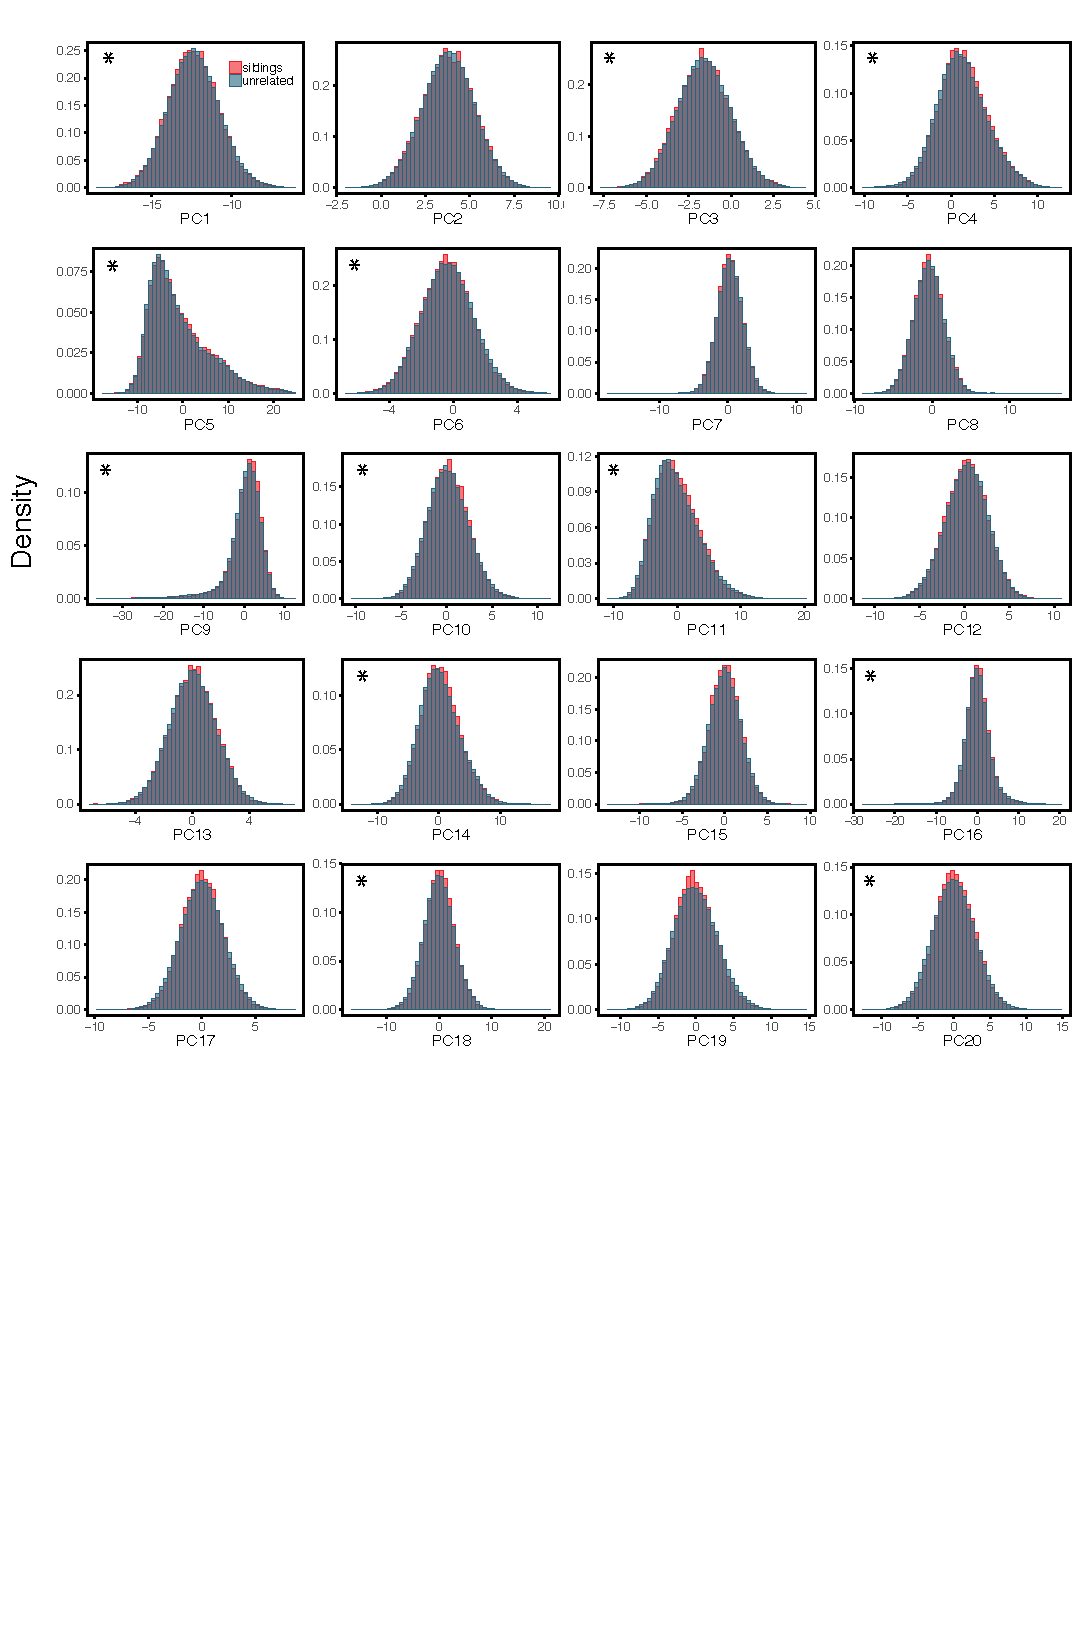
\includegraphics[width=\textwidth]{./supp_figures/sibs_unrel_compare2.pdf}
\caption{sibs vs unrel: PCs}
\end{figure}

\begin{figure}[h!]
\centering
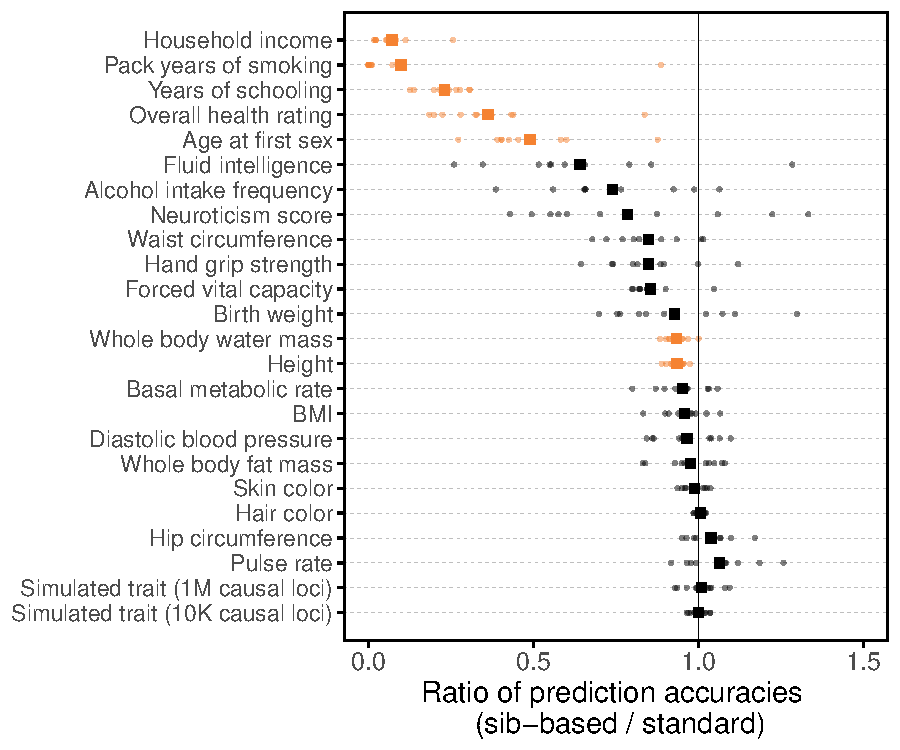
\includegraphics[width=10cm]{./supp_figures/fig3_panelA_SI.pdf}
\caption{repeat of Fig 3 with residualized phenotypes}
\end{figure}

\begin{table}[h!]
\caption{List of traits analyzed}
\begin{center}
 \begin{tabular}{| l l |} 
 \hline
 \textbf{Trait} & \textbf{UKB data field} \\ [0.5ex] 
 \hline\hline
  Age at first sex & 2139  \\ 
  Alcohol intake frequency & 1558  \\
  Basal metabolic rate & 23105  \\ 
  Birth weight & 20022  \\ 
  Body mass index & 21001  \\
  Diastolic blood pressure & 4079, 6153, 6177  \\ 
  Fluid intelligence & 20016  \\ 
  Forced vital capacity & 3062  \\ 
  Hair color & 1747  \\ 
  Hand grip strength & 46, 47  \\ 
  Height & 50  \\ 
  Hip circumference & 49  \\ 
  Household income & 738  \\ 
  Neuroticism score & 20127  \\ 
  Overall health rating & 2178  \\ 
  Pack years of smoking & 20161  \\ 
  Pulse rate & 102  \\ 
  Skin color & 1717  \\ 
  Waist circumference & 48  \\ 
  Whole body fat mass & 23100  \\ 
  Whole body water mass & 23102  \\ 
  Years of schooling & 6138 \\ 
   \hline
 \end{tabular}
\end{center}
\end{table}


\begin{table}[h!]
\caption{Genetic correlations across strata}
\begin{center}
 \begin{tabular}{|c | c | c |} 
 \hline
 \textbf{Trait/characteristic} & \textbf{Pair of strata} & \textbf{Genetic correlation (s.e.)} \\ [0.5ex] 
 \hline\hline
   & (Q1,Q2) & 0.93 (0.036)  \\ 
   & (Q1,Q3) & 0.95 (0.035)  \\ 
 BMI/Age & (Q1,Q4) & 0.95 (0.039)  \\ 
   & (Q2,Q3) & 0.89 (0.032)  \\ 
   & (Q2,Q4) & 0.91 (0.036)  \\ 
   & (Q3,Q4) & 1.00 (0.040)  \\ 
 \hline\hline
  & (Q1,Q2) & 0.98 (0.054)  \\ 
  & (Q1,Q3) & 0.99 (0.067)  \\ 
 Years of schooling/SES & (Q1,Q4) & 0.93 (0.068)  \\ 
  & (Q2,Q3) & 0.97 (0.063)  \\ 
  & (Q2,Q4) & 1.09 (0.074)  \\ 
  & (Q3,Q4) & 1.04 (0.074)  \\ 
 \hline\hline
 DBP/Sex & (male,female) & 0.93 (0.031)  \\ 
 \hline
 \end{tabular}
 \end{center}
\end{table}


\begin{table}[h!]
\caption{Sample sizes for sibling and unrelated sets}
\begin{center}
\small
 \begin{tabular}{| l l l l l |} 
 \hline
 \textbf{Trait} & \textbf{Siblings (pairs)} & \textbf{Unrelateds-discovery} & \textbf{Unrelateds-n*} & \textbf{Unrelateds-prediction}\\ [0.5ex] 
 \hline\hline
  Age at first sex & 13677 & 244929 & 8843 & 27214 \\
Alcohol intake frequency & 17288 & 276872 & 10977 & 30763 \\
Basal metabolic rate & 16802 & 269728 & 13490 & 29969 \\
Birth weight & 6753 & 159237 & 5608 & 17693 \\
Body mass index & 17223 & 274887 & 12377 & 30543 \\
Diastolic blood pressure & 14795 & 253343 & 9424 & 28149 \\
Fluid intelligence & 3889 & 101070 & 2928 & 11229 \\
Forced vital capacity & 14611 & 252859 & 9731 & 28095 \\
Hair color & 16859 & 272151 & 11825 & 30238 \\
Hand grip strength & 17070 & 275067 & 10884 & 30563 \\
Height & 17248 & 270065 & 18085 & 30007 \\
Hip circumference & 17254 & 275957 & 11615 & 30661 \\
Household income & 13244 & 239274 & 8787 & 26585 \\
Neuroticism score & 11759 & 227111 & 6825 & 25234 \\
Overall health rating & 17195 & 276628 & 10365 & 30736 \\
Pack years of smoking & 2307 & 85626 & 1604 & 9513 \\
Pulse rate & 14791 & 253877 & 8790 & 28208 \\
Skin color & 16903 & 274150 & 10342 & 30461 \\
Waist circumference & 17257 & 275863 & 11757 & 30651 \\
Whole body fat mass & 16750 & 270569 & 12046 & 30063 \\
Whole body water mass & 16804 & 269694 & 13535 & 29965 \\
Years of schooling & 17041 & 273599 & 11873 & 30399 \\
   \hline\hline
Simulated trait 1 & 17305 & 276731 & 11362 & 30747 \\
Simulated trait 2 & 17305 & 276382 & 11749 & 30709 \\
   \hline
 \end{tabular}
\end{center}
\end{table}


\begin{table}[h!]
\caption{Degree conversion table}
\begin{center}
 \begin{tabular}{| l l |} 
 \hline
 \textbf{Qualifications (UKB data field 6138)} & \textbf{Years of schooling} \\ [0.5ex] 
 \hline\hline
  College or University degree  & 20  \\ 
  NVQ or HND or HNC or equivalent & 19  \\
  Other professional qualifications eg: nursing, teaching  & 15  \\
  A levels/AS levels or equivalent & 13  \\
  O levels/GCSEs or equivalent  & 10  \\
  CSEs or equivalent & 10  \\
  None of the above & 7  \\
   \hline
 \end{tabular}
\end{center}
\end{table}


%\subsubsection{Consequences of direct-indirect correlation and significance threshold}
%\hl{to be completed}
%
%To gain some intuition we first note that \hl{[discuss with derivatives assuming fixed contribution across sites, add plot]} if indirect effects are strongly positively correlated with direct effects then prediction accuracy would be higher for standard GWAS than sib-regression.
%
%We next look at the effect of changing the significance threshold on SNPs (in the ascertainment set) that we include in our standard and sib-based polygenic scores.  We can rewrite eq.~\ref{R_indirect_general_form} as follows
%$$R=\frac{\sum_i^mA(i)}{\sqrt{\sum_i^mB(i)}},$$
%with
%$$A(i):=Var[x_i](\beta_i+\eta_i)E[\hat{\beta}_i]$$
%and
%$$B(i)=Var[y]Var[\hat{\beta}_i]E[x_i^2]+\sum_i^mVar[x_i]E[\hat{\beta}_i]^2$$
%being positive. We will approximate the effect of changing the p-value threshold as a change to the number of SNPs in the polygenic score ($m$).  The change in prediction accuracy as we change $m$ is
%$$\frac{dR}{\partial	m}=\frac{A(m)\sum_i^mB(i)+B(m)\sum_i^mA(i)}{(\sum_i^mB(i))^{\frac{3}{2}}}=(\frac{A(m)}{\sum_i^mA(i)}+\frac{B(m)}{\sum_i^mB(i)})R$$

% we fix $Var[x_i]$, $\beta_i$ and $\eta_i$ across all sites $i$, then $R_{ur}-R_{sib}$ is monotonically increasing with $\eta_i$.  This suggests to us that indirect effects that are positively correlated with direct effects give higher prediction accuracy for standard GWAS than sib-regression.  This also suggests that in the case of indirect effects tending to have the opposite sign, $R$ may even be negative for sib regression.
%\cite{Bischoff2006}
\pagebreak

\bibliographystyle{acm}

%\bibliography{sample_size_matching}

\end{document}

